\documentclass[12pt,a4paper,oneside]{report}

\usepackage[a4paper,margin=1in]{geometry}
\usepackage[T1]{fontenc}
\usepackage[utf8]{inputenc}
\usepackage{lmodern}
\usepackage{setspace}
\usepackage{graphicx}
\usepackage{booktabs}
\usepackage{array}
\usepackage{tabularx}
\usepackage{longtable}
\usepackage{float}
\usepackage{tikz}
\usetikzlibrary{arrows.meta}
\usepackage{caption}
\usepackage{hyperref}
\usepackage{titlesec}
\usepackage{xcolor}
\usepackage[protrusion=true,expansion=false]{microtype}

\hypersetup{
    colorlinks=true,
    linkcolor=black,
    urlcolor=black,
    citecolor=blue
}

\setstretch{1.25}
\captionsetup[figure]{skip=8pt}
\setcounter{secnumdepth}{3}
\setcounter{tocdepth}{3}

\titleformat{\chapter}[display]
  {\centering\bfseries}
  {\Large Chapter \thechapter}
  {0.5em}
  {\Large}

\titleformat{name=\chapter,numberless}[display]
  {\centering\bfseries\Large}
  {}
  {0pt}
  {}

\titlespacing*{\chapter}{0pt}{-12pt}{24pt}
\titlespacing*{\section}{0pt}{18pt}{7pt}
\titlespacing*{\subsection}{0pt}{14pt}{5pt}

\newcommand{\ReportTitle}{Distributed Edge AI for Cooperative Perception in Autonomous Vehicles}
\newcommand{\DegreeName}{Bachelor of Technology}
\newcommand{\DepartmentName}{Computer Science \& Engineering}
\newcommand{\InstitutionName}{Barak Valley Engineering College}
\newcommand{\InstitutionAddress}{Nirala, Sribhumi -- 788701, Assam}
\newcommand{\GuideName}{Mr. N Rana Singha}
\newcommand{\GuideDesignation}{Assistant Professor, Department of Computer Science \& Engineering}
\newcommand{\SubmissionDate}{2026}
\newcommand{\AcademicSession}{2023--2027}
\newcommand{\StudentNames}{%
  \begin{enumerate}\setlength{\itemsep}{2pt}\setlength{\topsep}{4pt}
    \item Anirban Saikia (232010007005)
    \item Avirup Roy (232010007010)
    \item Ritesh Kumar Das (232010007046)
    \item Hijbul Bahar Mazumder (242050007003)
    \item Syed Yashin Hussain (242050007014)
  \end{enumerate}%
}

\newcommand{\frontmatterchapter}[1]{%
  \chapter*{#1}%
  \addcontentsline{toc}{chapter}{#1}%
}

\renewcommand{\bibname}{References}

\newcommand{\InstitutionHeader}{%
  \begin{center}
    
\includegraphics[width=1.35in]{images/bvec_logo.png}\par
    \vspace{0.15cm}
    {\large\bfseries\color{red} Department of Computer Science \& Engineering\par}
    \vspace{0.12cm}
    {\Large\bfseries\color{blue} BARAK VALLEY ENGINEERING COLLEGE\par}
    \vspace{0.08cm}
    {\small (A Govt.\ of Assam Institution, Approved by AICTE, New Delhi, Govt.\ of India)\par}
    {\small District: Sribhumi, Assam, 788701\par}
  \end{center}
  \vspace{0.2cm}
  \hrule
  \vspace{0.55cm}
}

\newcommand{\CertificateHeading}[1]{%
  \begin{center}
    {\large\bfseries #1\par}
  \end{center}
  \vspace{0.8cm}
}

\AddToHook{shipout/background}{%
  \pdfliteral page{q 0 G 0.4 w 25.2 25.2 544.88 791.49 re S Q}%
}

\begin{document}

\begin{titlepage}
    \newgeometry{top=0.7in,bottom=0.4in,left=1in,right=1in}
    \centering
    \setstretch{1.1}
    \vspace*{0.15cm}

    {\fontsize{22}{27}\selectfont\bfseries \ReportTitle\par}
    \vspace{1.0cm}

    {\large\itshape A Thesis (Major Project) submitted in partial fulfilment\\
    of the requirements\par}
    \vspace{0.8cm}

    {\large\itshape For the Degree of\\[0.15cm]
    \DegreeName\\[0.15cm]
    In\\[0.15cm]
    \normalfont\bfseries Computer Science and Engineering\par}
    \vspace{0.8cm}

    {\large Submitted by\par}
    \vspace{0.4cm}
    \begin{tabular}{ll}
      Anirban Saikia & (232010007005)\\
      Avirup Roy & (232010007010)\\
      Ritesh Kumar Das & (232010007046)\\
      Hijbul Bahar Mazumder & (242050007003)\\
      Syed Yashin Hussain & (242050007014)
    \end{tabular}
    \vspace{0.7cm}

    {\large Under the Guidance of\\[0.15cm]
    \textbf{\GuideName}\\
    \GuideDesignation\par}
    \vspace{0.7cm}
    
\includegraphics[width=1.4in]{images/bvec_logo.png}\par
    \vspace{0.15cm}

    {\large\bfseries DEPARTMENT OF COMPUTER SCIENCE \& ENGINEERING\\
    BARAK VALLEY ENGINEERING COLLEGE\\
    \normalsize NIRALA, SRIBHUMI -- 788701, ASSAM\\[0.25cm]
    \large \SubmissionDate\par}
\end{titlepage}
\restoregeometry

\pagenumbering{roman}

\frontmatterchapter{Declaration}

We, the students of \DepartmentName, \InstitutionName, declare that the
project report entitled \textbf{``\ReportTitle''} has been prepared under
the guidance of \textbf{\GuideName}, \DepartmentName, \InstitutionName.

\par\medskip

The report has been prepared without resorting to plagiarism. We have adhered
to the principles of academic honesty and integrity. No falsified or
fabricated data have been presented in this report. Further, the matter
embodied in this project report has not been submitted previously for the
award of any degree or diploma.

\vspace{0.8cm}

\noindent
Anirban Saikia (232010007005)\\[0.2cm]
Avirup Roy (232010007010)\\[0.2cm]
Ritesh Kumar Das (232010007046)\\[0.2cm]
Hijbul Bahar Mazumder (242050007003)\\[0.2cm]
Syed Yashin Hussain (242050007014)

\vfill

\noindent
Date: \rule{4cm}{0.4pt}\\[0.2cm]
Place: \rule{4cm}{0.4pt}

\clearpage
\thispagestyle{plain}
\phantomsection
\addcontentsline{toc}{chapter}{Certificate of Approval}
\InstitutionHeader
\CertificateHeading{CERTIFICATE OF APPROVAL}

\noindent
\textbf{Project Title:} \ReportTitle\\
\textbf{Project Category:} Major Project Report\\
\textbf{Student Names:}

\StudentNames

\noindent
\textbf{Name of the Department:} Computer Science \& Engineering\\
\textbf{Name of the Supervisor:} \GuideName\\
\textbf{Academic Session:} \AcademicSession\\
\textbf{Recommendation:} [-]

\vfill

\noindent
\textbf{Dr. Kausthav Pratim Kalita}\\
Head, Department of Computer Science \& Engineering\\
Barak Valley Engineering College

\clearpage
\thispagestyle{plain}
\phantomsection
\addcontentsline{toc}{chapter}{Certificate from External Examiner}
\InstitutionHeader
\CertificateHeading{CERTIFICATE FROM EXTERNAL EXAMINER}

This is to certify that I have examined the major project report entitled
``\ReportTitle'', submitted by the following students of Bachelor of
Technology in Computer Science and Engineering:

\StudentNames

The report submitted to the Department of Computer Science \& Engineering,
Barak Valley Engineering College, Sribhumi, Assam, in partial fulfilment of
the requirements for the award of the degree of Bachelor of Technology in
Computer Science and Engineering, has been examined by me and found to be
satisfactory.

\vfill

\noindent
\begin{minipage}[t]{0.48\textwidth}
  Date: \rule{4cm}{0.4pt}\\[0.2cm]
  Place: \rule{4cm}{0.4pt}
\end{minipage}\hfill
\begin{minipage}[t]{0.40\textwidth}
  \centering
  \rule{5cm}{0.4pt}\\[0.2cm]
  External Examiner
\end{minipage}

\clearpage
\thispagestyle{plain}
\phantomsection
\addcontentsline{toc}{chapter}{Certificate from Supervisor}
\InstitutionHeader
\CertificateHeading{CERTIFICATE FROM SUPERVISOR}

This is to certify that the major project/thesis work embodied in this report
entitled ``\ReportTitle'', submitted by:

\StudentNames

of Bachelor of Technology in the Department of Computer Science \& Engineering
is based on their work under my supervision and is prepared for their academic
requirements. It is also certified that this work has not been submitted
elsewhere for any degree or diploma.

\vfill

\noindent
\begin{minipage}[t]{0.45\textwidth}
  Date: \rule{4cm}{0.4pt}\\[0.2cm]
  Place: \rule{4cm}{0.4pt}
\end{minipage}\hfill
\begin{minipage}[t]{0.48\textwidth}
  \raggedleft
  \textbf{\GuideName}\\
  Assistant Professor\\
  Department of Computer Science \& Engineering
\end{minipage}

\clearpage
\frontmatterchapter{Abstract}

Autonomous vehicles rely on timely onboard AI to interpret camera, LiDAR,
and radar data, yet an individual vehicle's sensors can be limited by range
and occlusion. This report reviews distributed Edge AI for autonomous
vehicles and records initial CARLA implementation and evaluation progress.
The literature motivates a vehicle--edge--cloud architecture with onboard
perception, optional V2V/V2I cooperation, and cloud services for longer-term
training and management; network services are not a safety-critical
dependency. Implemented CARLA work so far includes projecting simulator
ground-truth labels into camera images in four weather conditions, recording
a three-camera driving dataset, benchmarking a YOLO detector, and training
two PilotNet-style steering runs on autopilot data. In the 198-frame GPU
FP32 detector test, end-to-end latency averaged 20.5 ms (p95 24.2 ms).
However, the saved seed-0 steering run did not outperform the
always-straight baseline: its final validation MAE was 0.0863, its lowest
validation MAE occurred at epoch 1, and turn direction matched in 49\% of
turn cases. These are simulator-specific preliminary measurements; the
current implementation does not yet demonstrate cooperative V2V fusion,
edge offloading, or real-vehicle safety.

\par\medskip
\noindent\textbf{Keywords:} Distributed Edge AI, Autonomous Vehicles,
Cooperative Perception, V2X, Communication-Efficient Inference

\clearpage
\frontmatterchapter{Acknowledgement}

\noindent
We would like to extend our sincere thanks to all those who helped us
prepare this report. Without their guidance, support, cooperation, and
encouragement, we would not have been able to complete it successfully.

\par\noindent
\hspace*{1em}We express our sincere gratitude to our project guide,
\textbf{\GuideName}, for valuable guidance, support, and encouragement
throughout this work.

\par\noindent
\hspace*{1em}We also thank the faculty members of the Department of Computer
Science \& Engineering, Barak Valley Engineering College, for their
suggestions and academic support.

\vspace{0.8cm}
\begin{flushright}
  \rule{4cm}{0.4pt}\\[-0.05cm]
  Anirban Saikia (232010007005)\\[0.5cm]
  \rule{4cm}{0.4pt}\\[-0.05cm]
  Avirup Roy (232010007010)\\[0.5cm]
  \rule{4cm}{0.4pt}\\[-0.05cm]
  Hijbul Bahar Mazumder (242050007003)\\[0.5cm]
  \rule{4cm}{0.4pt}\\[-0.05cm]
  Ritesh Kumar Das (232010007046)\\[0.5cm]
  \rule{4cm}{0.4pt}\\[-0.05cm]
  Syed Yashin Hussain (242050007014)
\end{flushright}

\vfill
\noindent
Date: \rule{4cm}{0.4pt}\\[0.2cm]
Place: \rule{4cm}{0.4pt}

\clearpage
\tableofcontents
\clearpage
\listoftables
\clearpage
\listoffigures
\clearpage

\pagenumbering{arabic}

\chapter{Introduction}

Autonomous vehicles must interpret camera, LiDAR, radar, and other sensor
data in time to support driving functions. A vehicle's onboard perception
can also be limited by sensor range, occlusion, and constrained compute,
memory, power, and thermal resources. Sharing selected observations with
nearby vehicles may supplement an ego vehicle's view, but network delay and
interruption mean that local perception must remain available.

Distributed Edge Artificial Intelligence studies how AI workloads can be
placed across resource-constrained end devices, nearby edge servers, and
cloud infrastructure. Rather than treating every device as an independent
system, distributed approaches allow multiple nodes to contribute to
training, inference, or other application tasks. This report focuses on
cooperative perception as its primary online workload: connected vehicles
share selected observations or representations to address limitations in
each vehicle's local view. The design must determine what information to
exchange and where to align and fuse it while accounting for the different
capabilities and connectivity of vehicles, roadside edge servers, and cloud
resources.

\begin{figure}[H]
  \centering
  \resizebox{0.98\linewidth}{!}{%
    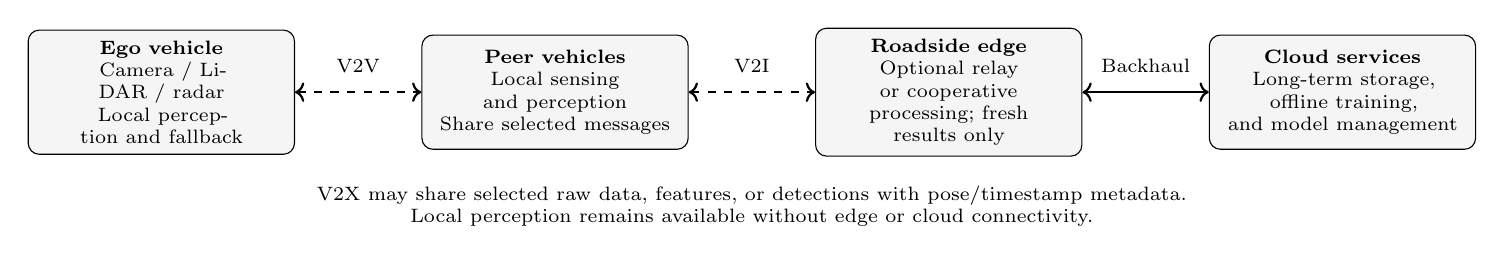
\begin{tikzpicture}[
      font=\scriptsize,
      nodebox/.style={draw, rounded corners, fill=gray!8, align=center,
        text width=3.1cm, minimum height=1.45cm, inner sep=4pt},
      v2x/.style={<->, dashed, thick},
      backhaul/.style={<->, thick}
    ]
      \node[nodebox] (ego) at (0,0)
        {\textbf{Ego vehicle}\\Camera / LiDAR / radar\\
        Local perception and fallback};
      \node[nodebox] (peers) at (5.0,0)
        {\textbf{Peer vehicles}\\Local sensing and perception\\
        Share selected messages};
      \node[nodebox] (edge) at (10.0,0)
        {\textbf{Roadside edge}\\Optional relay or cooperative\\
        processing; fresh results only};
      \node[nodebox] (cloud) at (15.0,0)
        {\textbf{Cloud services}\\Long-term storage, offline training,\\
        and model management};

      \draw[v2x] (ego.east) -- (peers.west)
        node[midway, above=2mm, fill=white, inner sep=1pt]
        {V2V};
      \draw[v2x] (peers.east) -- (edge.west)
        node[midway, above=2mm, fill=white, inner sep=1pt]
        {V2I};
      \draw[backhaul] (edge.east) -- (cloud.west)
        node[midway, above=2mm, fill=white, inner sep=1pt]
        {Backhaul};

      \node[align=center] at (7.5,-1.45)
        {V2X may share selected raw data, features, or detections with pose/timestamp metadata.\\
        Local perception remains available without edge or cloud connectivity.};
    \end{tikzpicture}%
  }
  \caption{Autonomous-Vehicle Cooperative Perception in a Distributed Edge Architecture.}
  \label{fig:distributed-edge-ai-overview}
\end{figure}

\section{Background}

Edge AI refers to executing artificial intelligence computations close to
the data source, at the network edge, rather than in a centralised cloud data
centre \cite{deng2020}. In an autonomous vehicle, sensors such as cameras,
radar, lidar, and positioning sensors provide inputs to onboard computing
units, which run perception and other latency-sensitive AI tasks. Nearby
roadside units or multi-access edge-computing servers can provide additional
compute capacity to connected vehicles, and cloud resources can provide
centralised storage and model-training services. These layers differ in
proximity, compute capacity, storage, and network connectivity. Work requiring an immediate response is therefore proposed to remain
onboard. Cooperative perception may exchange selected raw observations,
intermediate features, or compact detections with pose and timestamp
metadata. Other workloads may use edge or cloud resources subject to their
latency, bandwidth, privacy, and availability requirements
\cite{biswas2023}.

Edge intelligence encompasses both the use of AI to manage edge systems and
the execution of AI workloads on edge resources \cite{deng2020}. Distributed
Edge AI extends this setting by coordinating work across interconnected,
heterogeneous nodes. For example, a distributed scheduler can place
application tasks across edge nodes as system conditions change
\cite{hu2023}. In collaborative inference, a model's computation can be
partitioned so that multiple devices contribute to producing a result
\cite{hou2022}. These approaches make task placement and coordination
important parts of the system design.

The choice of where to execute a workload affects more than processing
speed. Sending data or intermediate model outputs across a network consumes
bandwidth and introduces communication delay; keeping computation local can
reduce some transfers but is constrained by device capacity and energy
availability. Federated learning offers a way for clients to train
collaboratively without collecting their raw training data at one central
location, while still requiring the exchange and coordination of model
updates \cite{deng2020}. Partitioned inference, in turn, must balance local
computation against the cost of transferring intermediate results
\cite{hou2022}.

There is no single placement strategy that fits every workload. A design
that is appropriate for a delay-sensitive application may not be optimal
when energy, network availability, or device diversity is the main
constraint. Distributed systems must account for communication cost,
heterogeneous computing resources, changing node availability, and the
privacy and security implications of sharing data or model information
\cite{deng2020,hu2023}. This report applies these considerations to
autonomous vehicles. Vehicle sensors generate high-volume, time-varying
inputs; onboard computing must support timely perception despite limited
resources; roadside edge servers may be intermittently reachable; and cloud
resources are remote. The architecture must therefore decide which AI
workloads remain local and which can be shared or offloaded without making
immediate driving decisions dependent on a network connection
\cite{biswas2023,deng2020}.

\section{Problem Statement}

The central problem is how cooperative perception can combine selected
information from multiple connected vehicles or roadside infrastructure to
improve an ego vehicle's view while accounting for communication overhead,
latency, freshness, and heterogeneous agents. Onboard processing must
continue immediate local perception, but is bounded by compute, memory,
energy, and thermal capacity. V2V/V2I sharing can add complementary
observations, while intermittent links and network cost constrain what can
be exchanged. Roadside offloading is considered a supporting option; cloud
execution supports longer-term services and is not assumed for immediate
safety-critical decisions. The project will compare perception quality
against communication, resource, energy, and reliability costs.

This report examines these trade-offs through a literature review and
preliminary CARLA experiments. Initial data-capture, detection, and steering
experiments have been implemented, but cooperative information exchange and
fusion have not yet been demonstrated. The available measurements
characterize the current single-vehicle simulation prototype, not a
distributed system. The project is guided by two questions: how can
multiple agents' selected sensor-derived information be aligned and fused
without making immediate local processing depend on connectivity; and what
communication, latency, freshness, quality, hardware, and reliability
measures should inform a feasible prototype?

\section{Objectives}

The objectives of this preliminary study are:
\begin{enumerate}
  \item Study distributed Edge AI architectures and their applicability to
  autonomous-vehicle cooperative perception.
  \item Investigate cooperative perception among vehicles, including
  feature sharing, fusion, and communication-aware inference.
  \item Analyze communication latency, compute and memory constraints,
  bandwidth, energy use, and reliability.
  \item Propose a distributed Edge AI architecture for multi-agent
  autonomous-vehicle perception, with edge offloading as a supporting option.
  \item Develop a feasibility-assessment and evaluation framework for a
  future prototype.
  \item Conduct initial CARLA data-capture, perception-latency, and
  steering-baseline experiments, and use their limitations to guide the
  small-scale experimental phase.
\end{enumerate}

\section{Scope and Report Organization}

This report combines a literature review with preliminary CARLA experiments.
The current single-vehicle pipeline projects ground-truth labels, records
three camera views, benchmarks YOLO detection, and tests PilotNet-style
steering. It has not implemented V2V exchange, cooperative fusion, or edge
offloading. Hardware, software, and model details remain to be documented
for reproducibility. Chapter 2 surveys the literature
and vehicle workloads; Chapter 3 describes the proposed distributed
architecture and initial CARLA pilot; Chapter 4 presents literature
findings and measured CARLA results; and Chapter 5 summarizes limitations
and next steps. Federated learning remains a secondary literature topic.

The project follows a six-phase research and development process: (1)
learning the fundamentals of Edge AI and autonomous-vehicle systems, (2)
reviewing literature on cooperative perception and communication, (3)
conducting small-scale experiments, (4) assessing the
feasibility of a cooperative vehicle--edge prototype, (5) implementing the
selected system, and (6) testing and refining it. At the current stage, the
project is entering Phase 3, Small-Scale Experiments. Initial CARLA
simulation and data gathering provide a starting point for this phase.
Multi-agent cooperative perception, V2X integration, and comparative
distributed evaluation remain future work; the current pilot does not
complete Phase 3 or the later implementation and testing phases. The overall
plan and current stage are summarised in
Figure~\ref{fig:six-phase-research-plan}.

\begin{figure}[H]
  \centering
  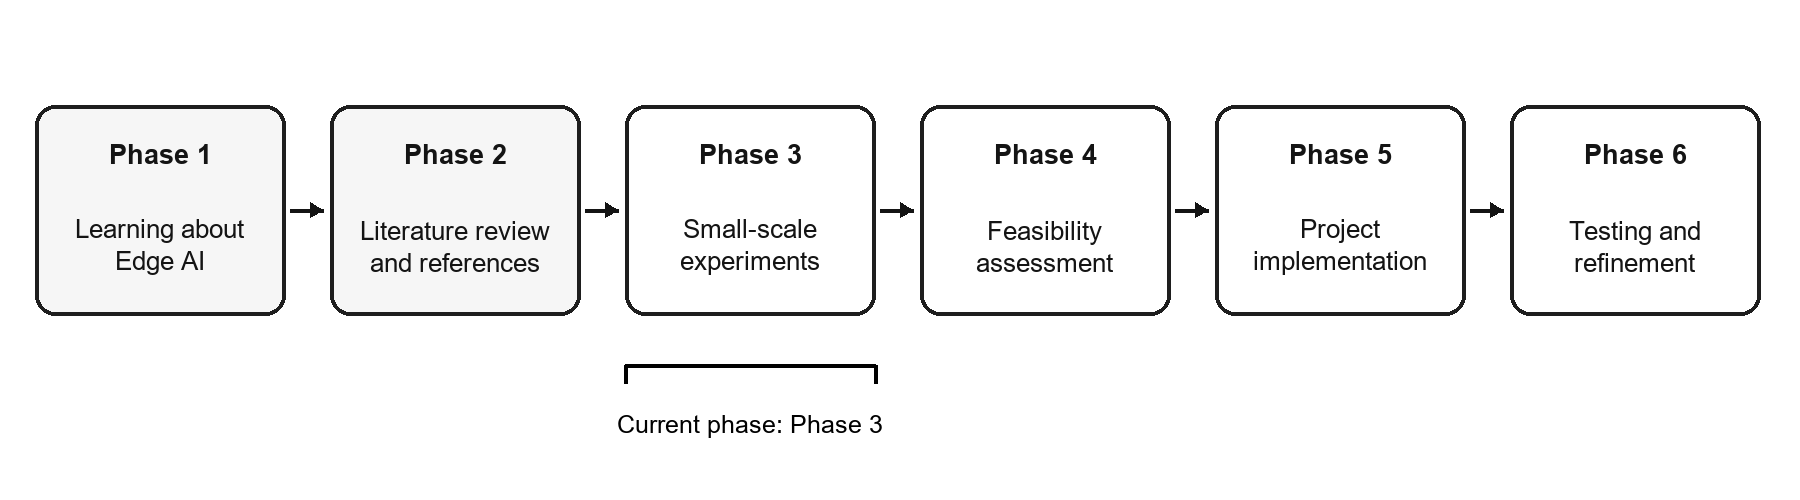
\includegraphics[width=0.94\linewidth]{images/six-phase-research-plan.png}
  \caption{Six-Phase Research and Development Plan.}
  \label{fig:six-phase-research-plan}
\end{figure}

\chapter{Literature Survey}

\section{From Cloud AI to Edge Intelligence}

The reviewed literature positions distributed edge AI as a response to the
limits of centralised cloud processing. Edge AI performs AI computation near
the user at the network edge rather than in a centralised data centre; this
shift has been enabled by improvements in AI efficiency, the proliferation of
IoT devices, and the growth of edge computing. Zhou et al.\ describe edge
intelligence as extending AI to the ``last mile'' for mobile and IoT devices
that generate data at the edge. Deng et al.\ distinguish AI for edge from
AI on edge, with the latter covering model training and inference on edge
devices \cite{deng2020}. The term ``edge'' has no universally accepted
definition; its relation to cloud computing depends on proximity, capacity,
and device heterogeneity \cite{deng2020}.

For autonomous vehicles, moving selected computation closer to the vehicle
can reduce reliance on distant cloud processing and enable cooperation with
nearby infrastructure. Edge intelligence is relevant to connected-vehicle
systems because it links vehicle sensing and onboard processing with
roadside and network resources. This potential does not remove the need for
local processing: changing connectivity and strict response requirements
make it important to keep immediate perception and control available within
the vehicle \cite{biswas2023}.

\section{End-Edge-Cloud Architectures}

A common architectural pattern distributes processing across end devices,
edge servers, and the cloud. In the vehicle setting, the vehicle is the end
device: it acquires sensor data and performs onboard perception. Roadside
units or nearby multi-access edge-computing servers provide additional,
lower-latency resources when reachable, while cloud infrastructure supports
central storage and large-scale services. End devices handle local
computation, while edge servers provide nearby, more capable resources.
The literature distinguishes the complementary roles of AI for edge and AI
on edge, and describes orchestration of heterogeneous on-device, edge,
and cloud resources for distributed AI. Collaborative learning across
cloud and edge resources is also studied \cite{deng2020}. Hu et al.\ describe
a distributed edge-AI scheduler that places application tasks across
heterogeneous nodes while accounting for changing system conditions
\cite{hu2023}. The layers and their data and model flows are summarised in
Figure~\ref{fig:vehicle-edge-cloud-overview}, which shows vehicle, peer,
roadside-edge, and cloud responsibilities. The V2V, V2I, and edge-to-cloud
communication paths and representative messages are shown separately in
Figure~\ref{fig:vehicle-communication-links}.

\section{Distributed Training: Federated Learning}

Federated learning (FL) trains local models on multiple clients without
collecting raw user data at a central data centre. Federated learning
and knowledge distillation are described as training approaches, while model
splitting and partitioning support inference. FL challenges include
statistical heterogeneity, communication cost, resource allocation, and
privacy and security. Communication can dominate computation when local
datasets are small and participant processors are comparatively fast
\cite{deng2020}. Figure~\ref{fig:federated-learning-workflow} illustrates
the local-training and model-aggregation workflow.

Communication efficiency, resource allocation, and data heterogeneity are
recurring concerns in distributed edge learning \cite{deng2020}.
McMahan et al.\ present federated averaging, in which clients perform local
training and a server averages their model updates. Their evaluation covers
five model architectures and four datasets, and reports 10--100 times fewer
communication rounds than synchronized stochastic gradient descent in the
settings tested \cite{mcmahan2017}. This result is specific to their
workloads and baselines; it does not imply the same reduction for every
edge-learning system.

Chellapandi et al.\ review federated-learning approaches for connected and
automated vehicles, including centralized and decentralized coordination,
vehicle data sources, model and application choices, and privacy and
security techniques \cite{flcav2024}. The survey identifies the potential
to learn across diverse driving environments without centralizing raw
vehicle data, while emphasizing communication overhead, client and data
heterogeneity, and security as open challenges. It is a literature survey,
not a new cooperative-perception benchmark. Federated learning therefore
remains relevant to future model development, but is secondary to this
project's online cooperative-perception workload.

In a vehicle deployment, participating vehicles could train locally from
their own collected data and coordinate model updates with roadside or
cloud infrastructure. Such collaboration could broaden the training data
available to a model without routinely uploading raw sensor recordings.
However, vehicle mobility and intermittent connections complicate
participant availability and synchronization; non-IID routes and driving
conditions can yield different local data distributions; and exchanged
updates still consume bandwidth and may expose information or be
manipulated. Federated training is an offline or periodic model-improvement
approach here, not a substitute for onboard inference or a mechanism for
making immediate driving decisions \cite{deng2020,biswas2023}.

\begin{figure}[H]
  \centering
  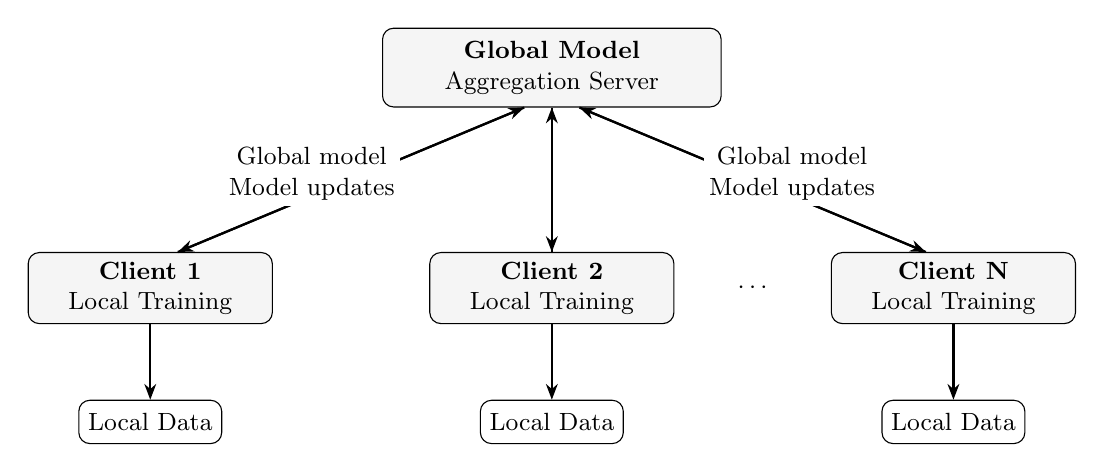
\begin{tikzpicture}[
    font=\small,
    flow/.style={-{Stealth[length=2mm]}, thick},
    client/.style={draw, rounded corners, fill=gray!8,
      minimum width=3.1cm, minimum height=0.85cm, align=center},
    data/.style={draw, rounded corners, minimum width=1.8cm,
      minimum height=0.55cm, align=center}
  ]
    \node[draw, rounded corners, fill=gray!8, minimum width=4.3cm,
      minimum height=1cm, align=center] (server) at (0,3.5)
      {\textbf{Global Model}\\Aggregation Server};
    \node[client] (client1) at (-5.1,0.7)
      {\textbf{Client 1}\\Local Training};
    \node[client] (client2) at (0,0.7)
      {\textbf{Client 2}\\Local Training};
    \node[client] (clientn) at (5.1,0.7)
      {\textbf{Client N}\\Local Training};
    \node[data] (data1) at (-5.1,-1.0) {Local Data};
    \node[data] (data2) at (0,-1.0) {Local Data};
    \node[data] (datan) at (5.1,-1.0) {Local Data};

    \draw[flow] ([xshift=-0.35cm]server.south) -- ([xshift=0.35cm]client1.north);
    \draw[flow] ([xshift=0.35cm]client1.north) -- ([xshift=-0.35cm]server.south);
    \draw[flow] (server.south) -- (client2.north);
    \draw[flow] (client2.north) -- (server.south);
    \draw[flow] ([xshift=0.35cm]server.south) -- ([xshift=-0.35cm]clientn.north);
    \draw[flow] ([xshift=-0.35cm]clientn.north) -- ([xshift=0.35cm]server.south);
    \node[draw=none, fill=white, inner sep=2pt, align=center]
      at (-3.05,2.15) {Global model\\Model updates};
    \node[draw=none, fill=white, inner sep=2pt, align=center]
      at (3.05,2.15) {Global model\\Model updates};
    \node at (2.55,0.7) {$\cdots$};
    \draw[flow] (client1.south) -- (data1.north);
    \draw[flow] (client2.south) -- (data2.north);
    \draw[flow] (clientn.south) -- (datan.north);
  \end{tikzpicture}
  \caption[Federated Learning Workflow]{Federated Learning Workflow. Adapted from Deng et al.\ \cite{deng2020}.}
  \label{fig:federated-learning-workflow}
\end{figure}

\section{Distributed Inference and Cooperative Perception}

\subsection{Single-model inference partitioning}

Model-partition methods split a deep neural network between a device and
server based on transmission latency and device energy. Early-exit methods
can reduce communication when intermediate features are sufficient.
DistrEdge applies deep reinforcement learning to distribute CNN inference
across heterogeneous IoT edge devices and reports a 1.1--3$\times$ speedup
over the state-of-the-art baselines evaluated in that study; this is a
study-specific result rather than a general speedup guarantee
\cite{hou2022}. The device--server split is shown in
Figure~\ref{fig:partitioned-collaborative-inference}.

\begin{figure}[H]
  \centering
  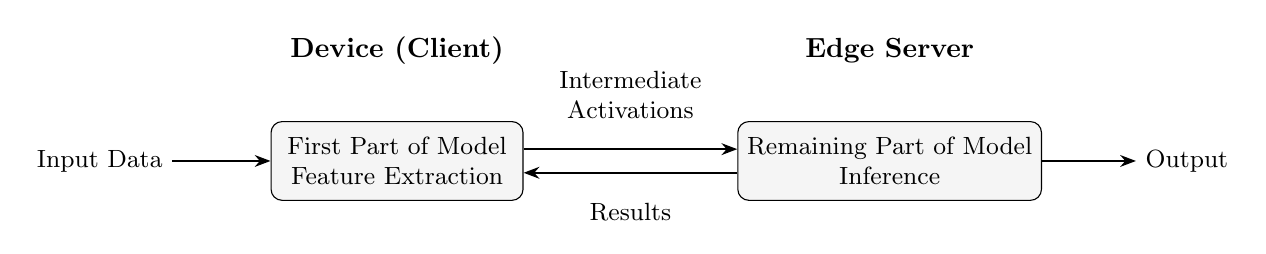
\begin{tikzpicture}[
    x=0.68cm,
    font=\small,
    flow/.style={-{Stealth[length=2mm]}, thick},
    block/.style={draw, rounded corners, fill=gray!8, align=center,
      minimum width=3.2cm, minimum height=1cm}
  ]
    \node[font=\bfseries] at (3.2,3.25) {Device (Client)};
    \node[font=\bfseries] at (12.4,3.25) {Edge Server};

    \node[block] (device) at (3.2,1.85)
      {First Part of Model\\Feature Extraction};
    \node[block] (edge) at (12.4,1.85)
      {Remaining Part of Model\\Inference};

    \draw[flow] (-1.0,1.85) -- (device.west);
    \node[left] at (-1.0,1.85) {Input Data};
    \draw[flow] ([yshift=0.15cm]device.east) -- ([yshift=0.15cm]edge.west)
      node[midway, above=3mm, fill=white, inner sep=2pt, align=center]
      {Intermediate\\Activations};
    \draw[flow] ([yshift=-0.15cm]edge.west) -- ([yshift=-0.15cm]device.east)
      node[midway, below=3mm, fill=white, inner sep=2pt, align=center] {Results};
    \draw[flow] (edge.east) -- (17.0,1.85);
    \node[right] at (17.0,1.85) {Output};
  \end{tikzpicture}
  \caption[Partitioned CNN Inference between a Device and Edge Server]{Partitioned CNN Inference between a Device and Edge Server. Adapted from Hou et al.\ \cite{hou2022}.}
  \label{fig:partitioned-collaborative-inference}
\end{figure}

\noindent
Hu et al.\ also describe a video-object-detection application divided into
frame extraction, object detection, and frame combination services
\cite{hu2023}. Figure~\ref{fig:distributed-video-object-detection} shows
this pipeline as a second example of distributed inference.
Assigning detection work to multiple containers can use available parallel
capacity and reduce frame-processing time up to a point. However, frames
and detection results must move between pipeline stages, adding network
traffic and communication delay; the reported benefit depends on the video
quality, container count, and deployment evaluated by Hu et al.\ \cite{hu2023}.

\begin{figure}[H]
  \centering
  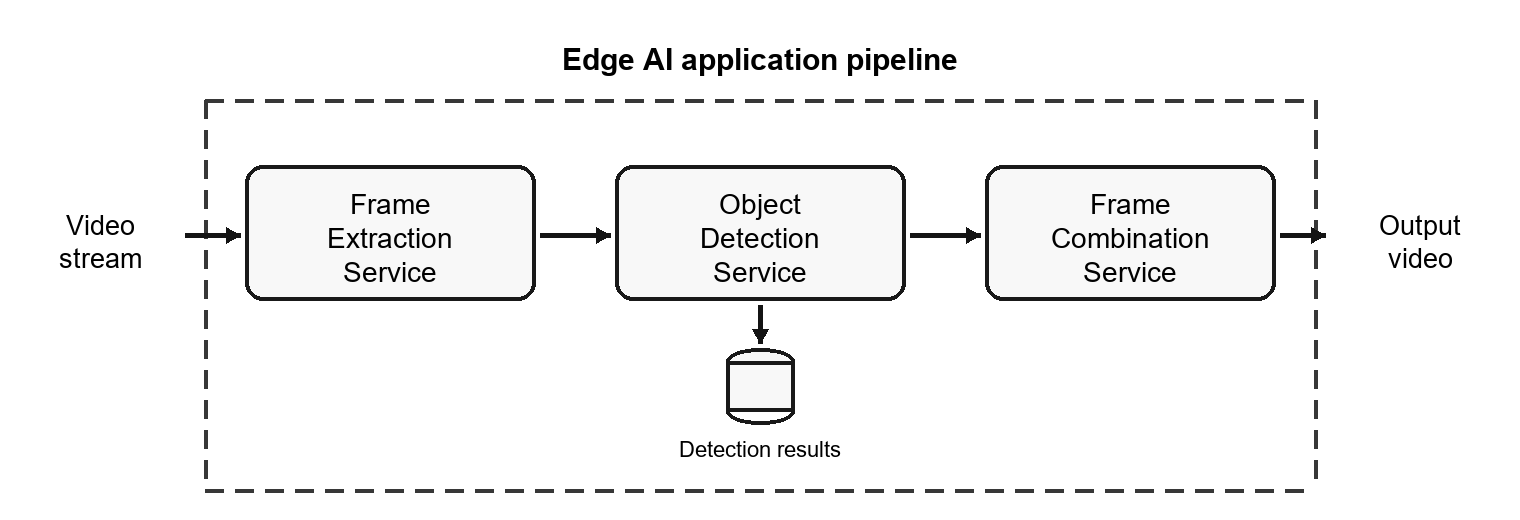
\includegraphics[width=\linewidth]{images/distributed-video-object-detection.png}
  \caption[Distributed Video Object-Detection Pipeline]{Distributed Video Object-Detection Pipeline. Adapted from Hu et al.\ \cite{hu2023}.}
  \label{fig:distributed-video-object-detection}
\end{figure}

\subsection{Multi-agent cooperative perception}

Cooperative perception addresses a different problem from partitioned
inference. It combines observations or learned representations from
multiple spatially separate vehicles; it does not necessarily split one
model's layers across a device and server. An ego vehicle can retain its
own perception path and fuse selected information from peers or
infrastructure to supplement occluded or distant regions. V2X-ViT and
CoBEVT study multi-agent fusion architectures, while Where2comm selects
spatially informative features to reduce communication
\cite{v2xvit2022,cobevt2023,where2comm2022}. Their simulated and benchmark
evaluations motivate a future comparison of ego-only and cooperative
perception, but do not validate the proposed system or a real vehicle
network.

For autonomous vehicles, onboard inference performs local detection,
classification, tracking, and environment perception. Cooperative
perception complements this local view by sharing sensor-derived
information between vehicles or with infrastructure and fusing it at an
ego vehicle or edge node. V2X-ViT uses heterogeneous multi-agent attention
and multi-scale window attention to fuse information from vehicles and
infrastructure; it evaluates LiDAR-based 3D detection on the simulated
V2XSet dataset; the authors report a 21.2\% AP gain over the single-agent
baseline and at least 7.3\% over the compared intermediate-fusion methods
\cite{v2xvit2022}. These figures are specific to their test protocol. Its
authors note simulation-to-reality and scalability limitations, as well as
privacy and adversarial-robustness concerns. CoBEVT instead uses sparse
fused axial attention to aggregate
multi-view camera features into cooperative bird's-eye-view maps. Its
evaluations on OPV2V and V2X-Sim report strong cooperative BEV segmentation
and extensions to multi-agent LiDAR 3D detection \cite{cobevt2023}. These
studies demonstrate research approaches on datasets, not validated
vehicle-road deployments. They motivate comparing ego-only perception
with cooperative feature fusion while retaining a local fallback.

\section{Communication Efficiency}

Communication is a central bottleneck across training and inference. What is
transmitted affects per-round overhead and the number of communication
rounds. Quantisation and pruning, together with in-network computation, are
discussed as ways to address communication cost. Computation-intensive
inference may require task splitting across edge devices and servers, making
communication efficiency especially important \cite{deng2020,hou2022}. In a
connected-vehicle setting, V2V links can carry cooperative perception
messages, while V2I links connect vehicles to roadside infrastructure.
Their delay, throughput, packet delivery, and availability can vary with
vehicle movement, obstruction, congestion, and radio conditions. A practical
design should therefore limit shared data to information useful to the
workload, account for message size and freshness, and measure network delay
and data volume alongside inference time. These communication links support
cooperation but are not assumed to be continuously available
\cite{biswas2023}.

Payload type is a key design choice. Raw camera frames or point clouds retain
more sensor detail but can require substantial bandwidth. Intermediate
features can reduce transmitted volume while preserving information useful
to a downstream model, but their size depends on the network and compression
scheme. Detection outputs and associated timestamps or poses are often
smaller, but discard information and can limit what a receiving agent can
infer. Where2comm addresses this trade-off with spatial confidence maps:
agents transmit sparse, perceptually important feature regions and adapt
the regions shared to available bandwidth. It evaluates camera and LiDAR
detection across vehicle and drone scenarios on OPV2V, V2X-Sim, DAIR-V2X,
and CoPerception-UAVs, measuring both average precision and communication
volume \cite{where2comm2022}. Its reported results are benchmark-specific;
the authors report over $100{,}000\times$ lower communication volume than
selected baselines while outperforming them on OPV2V. The approach focuses
on spatial selection, while temporal communication selection and deployment
over real wireless links remain further considerations. This work directly
motivates measuring payload bytes, perception quality, and latency together
in the proposed project.

\begin{figure}[H]
  \centering
  \resizebox{0.9\linewidth}{!}{%
    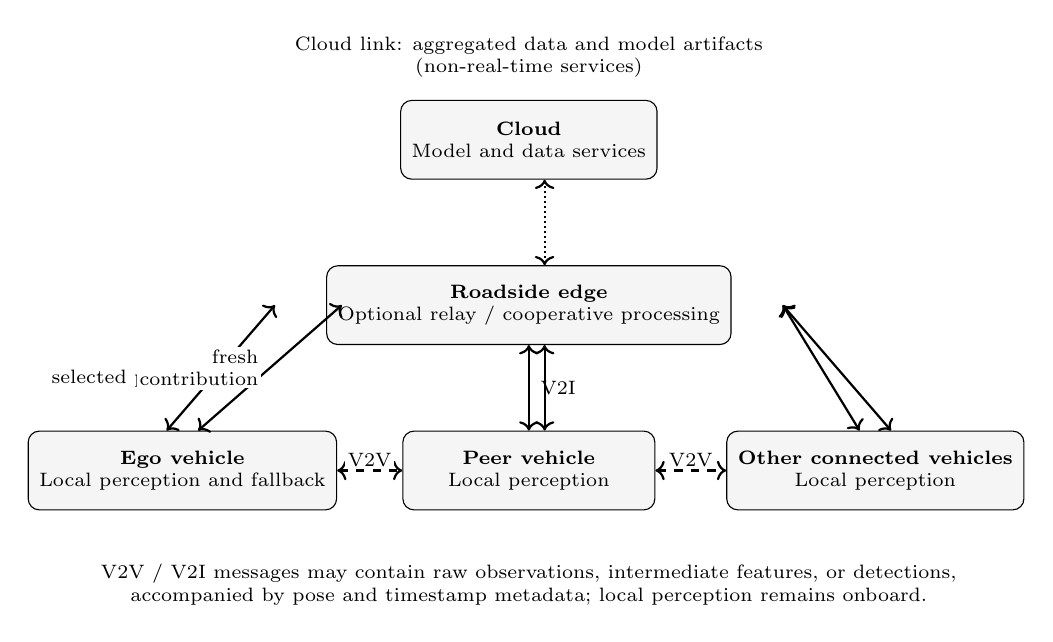
\begin{tikzpicture}[
      font=\scriptsize,
      nodebox/.style={draw, rounded corners, fill=gray!8, align=center,
        minimum width=3.2cm, minimum height=1.0cm, inner sep=4pt},
      v2v/.style={<->, dashed, thick},
      v2i/.style={<->, thick},
      backhaul/.style={<->, densely dotted, thick}
    ]
      \node[nodebox] (cloud) at (0,4.2)
        {\textbf{Cloud}\\Model and data services};
      \node[nodebox] (edge) at (0,2.1)
        {\textbf{Roadside edge}\\Optional relay / cooperative processing};
      \node[nodebox] (v1) at (-4.4,0)
        {\textbf{Ego vehicle}\\Local perception and fallback};
      \node[nodebox] (v2) at (0,0)
        {\textbf{Peer vehicle}\\Local perception};
      \node[nodebox] (vn) at (4.4,0)
        {\textbf{Other connected vehicles}\\Local perception};
      \draw[v2v] (v1.east) -- node[above, fill=white, inner sep=1pt]
        {V2V} (v2.west);
      \draw[v2v] (v2.east) -- node[above, fill=white, inner sep=1pt]
        {V2V} (vn.west);
      \draw[v2i] ([xshift=-0.2cm]v1.north) --
        ([xshift=-0.65cm]edge.west)
        node[midway, left=1mm, align=right, fill=white, inner sep=1pt]
        {V2I\\selected payload};
      \draw[v2i] ([xshift=0.2cm]edge.west) --
        ([xshift=0.2cm]v1.north)
        node[midway, left=1mm, align=right, fill=white, inner sep=1pt]
        {fresh\\contribution};
      \draw[v2i] (v2.north) -- (edge.south)
        node[midway, right=1mm, fill=white, inner sep=1pt] {V2I};
      \draw[v2i] ([xshift=0.2cm]edge.south) --
        ([xshift=0.2cm]v2.north);
      \draw[v2i] ([xshift=0.2cm]vn.north) --
        ([xshift=0.65cm]edge.east);
      \draw[v2i] ([xshift=0.65cm]edge.east) --
        ([xshift=-0.2cm]vn.north);
      \draw[backhaul] ([xshift=0.2cm]edge.north) --
        ([xshift=0.2cm]cloud.south);
      \node[align=center] at (0,5.25)
        {Cloud link: aggregated data and model artifacts\\
        (non-real-time services)};
      \node[align=center] at (0,-1.45)
        {V2V / V2I messages may contain raw observations, intermediate features, or detections,\\
        accompanied by pose and timestamp metadata; local perception remains onboard.};
    \end{tikzpicture}%
  }
  \caption{Vehicle Communication Links and Representative Cooperative-Perception Messages.}
  \label{fig:vehicle-communication-links}
\end{figure}

\section{Heterogeneity, Non-IID Data, and Stragglers}

FL over edge nodes must address device heterogeneity, non-independent and
identically distributed (non-IID) data, and limited communication resources.
Synchronous FL can wait for the slowest worker, while asynchronous FL may
cause frequent model transfers. The straggler effect can limit
synchronous training time. Non-IID and imbalanced data can cause local
updates to drift, resulting in instability and slower convergence; system
heterogeneity can also lead to stragglers and dropouts. Participant
selection is one proposed mitigation, while edge-assisted architectures,
data augmentation, and mediator-based rescheduling are reported as approaches
to non-IID bias. These challenges are part of the broader edge-intelligence
research landscape \cite{deng2020}. Vehicle fleets add hardware and
connectivity variation: vehicles may differ in accelerators, memory, sensor
suites, and available power, while their link quality and time within an
edge server's coverage change as they move. A collaborative method must not
assume uniform compute capacity or continuous participation; scheduling,
model selection, or fallback behavior should account for slower or
disconnected participants.

\section{Privacy and Security}

FL does not eliminate privacy risks: a malicious participant may infer
private data or poison a model. The surveyed literature discusses inference
attacks, honest-but-curious servers, free-riding participants, and
poisoning; differential privacy and other privacy-preserving approaches
involve design trade-offs \cite{deng2020}. Vehicle sensor streams can also
contain sensitive location and scene information, so sharing raw data,
features, or model updates requires privacy-aware handling. Connected
vehicle and roadside links additionally require authentication, integrity,
and protection against replay, spoofing, denial of service, and malicious
or compromised participants; these controls can add compute and
communication overhead. Security mechanisms and their impact on system
performance need to be evaluated together rather than assumed to eliminate
risk \cite{biswas2023}. Specific attack-success rates
are not reported here because the primary studies behind those figures
have not been verified for this review.

\section{Energy and Hardware Constraints}

Latency, energy use, memory footprint, and available computing resources
are relevant evaluation measures for edge workloads \cite{deng2020,hou2022}.
Their measured values depend on the device, model, network conditions, and
measurement setup. The cited DistrEdge evaluation, for example, does not
consider memory constraints and reports its speedups only against the
baselines and test cases used in that study \cite{hou2022}. A later
implementation should therefore record these conditions and avoid direct
comparison of results obtained under different protocols.
For vehicles, the available onboard compute may be constrained by the
installed processor or accelerator, memory, power budget, and heat
dissipation requirements. Sustained perception workloads can compete with
other onboard functions for these resources, so model size, frame rate,
energy use, and thermal behavior should be recorded on the selected
platform. Edge offloading can reduce local compute demand but adds network
and remote-resource dependencies; the vehicle must retain a local
capability for immediate processing \cite{biswas2023}.

\section{Application Domains}

Edge AI serves multiple domains, but this report focuses on autonomous
vehicles because sensor-driven perception combines substantial local
computation with stringent latency and connectivity constraints
\cite{biswas2023}. The following sections describe the vehicle system,
representative workloads, and vehicle--edge--cloud collaboration.

\section{Autonomous Vehicle Systems and Edge Intelligence}

Connected vehicles exchange information with other vehicles and
infrastructure; autonomous vehicles additionally use onboard sensing and
computation to interpret their surroundings and support driving functions.
The vehicle layer brings together cameras, radar, lidar, and positioning
sensors with onboard compute platforms. Sensor data can be high-volume and
time-sensitive, making local preprocessing and inference important both to
limit data movement and to support timely outputs. Edge infrastructure,
including roadside units or multi-access edge servers, can augment local
resources with cooperative processing when a low-latency connection is
available. Cloud services can support aggregated storage, model training,
and model distribution, but their remote connection is not a suitable
assumption for time-critical vehicle decisions \cite{biswas2023,deng2020}.

The relevant processing path has a real-time character: sensor inputs are
acquired, processed into a representation of the surrounding environment,
and used by downstream prediction or decision-support functions. The
acceptable delay and accuracy depend on the particular task and operating
conditions, and this report does not assign a universal deadline. The
proposed design therefore prioritizes local execution for immediate
perception and treats edge-assisted results as supplementary, with explicit
measurement of latency, availability, and fallback behavior
\cite{biswas2023,v2xvit2022,v2xsurvey2025}.

\begin{figure}[H]
  \centering
  \resizebox{0.95\linewidth}{!}{%
    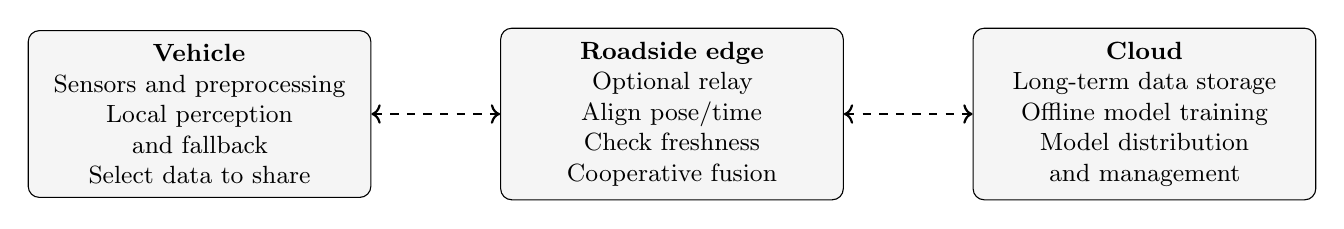
\begin{tikzpicture}[
      font=\small,
      layer/.style={draw, rounded corners, fill=gray!8, align=center,
        text width=4.0cm, minimum height=1.5cm, inner sep=5pt},
      optional/.style={<->, dashed, thick}
    ]
      \node[layer] (vehicle) at (0,0)
        {\textbf{Vehicle}\\Sensors and preprocessing\\
        Local perception\\and fallback\\Select data to share};
      \node[layer] (edge) at (6.0,0)
        {\textbf{Roadside edge}\\Optional relay\\
        Align pose/time\\Check freshness\\
        Cooperative fusion};
      \node[layer] (cloud) at (12.0,0)
        {\textbf{Cloud}\\Long-term data storage\\
        Offline model training\\
        Model distribution\\and management};
      \draw[optional] (vehicle.east) -- (edge.west);
      \draw[optional] (edge.east) -- (cloud.west);
    \end{tikzpicture}%
  }
  \caption{Functional Roles of Vehicle, Roadside-Edge, and Cloud Layers.}
  \label{fig:vehicle-edge-cloud-overview}
\end{figure}

\section{AI Workloads in Autonomous Vehicles}

An autonomous-vehicle AI pipeline can include sensor acquisition and
preprocessing, sensor synchronization and fusion, object detection and
classification, object tracking, environment perception, motion prediction,
and decision support. The exact sensors and models depend on the selected
vehicle platform and dataset; no specific model or hardware is fixed in
this report. Sensor fusion combines observations from available sources,
while detection and tracking estimate which objects are present and how
they move. These outputs can inform prediction and downstream driving
functions. The pipeline is shown as a conceptual workload sequence in
Figure~\ref{fig:autonomous-vehicle-ai-pipeline}.

OPV2V provides one candidate experimental resource for V2V cooperative
perception. The authors constructed 73 simulated scenes using CARLA and
OpenCDA, comprising 11,464 frames and 232,913 annotated 3D vehicle boxes;
the accompanying benchmark compares early, late, and intermediate fusion
strategies \cite{opv2v2022}. It provides a reproducible starting point for
testing perception and feature-sharing methods, but it is simulated data
and does not establish real-world radio performance or transfer to a
physical vehicle.

\begin{figure}[H]
  \centering
  \resizebox{0.98\linewidth}{!}{%
    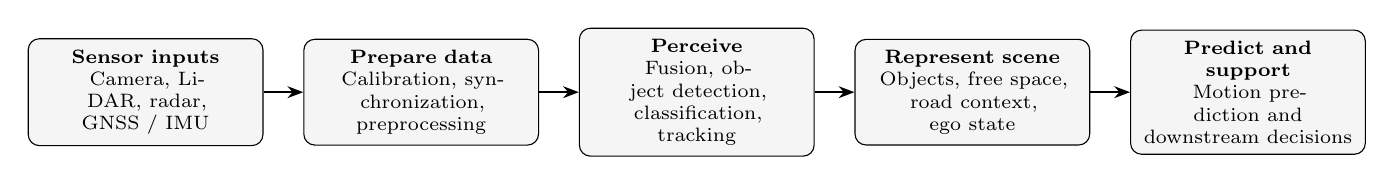
\begin{tikzpicture}[
      font=\scriptsize,
      stage/.style={draw, rounded corners, fill=gray!8, align=center,
        text width=2.7cm, minimum height=1.1cm, inner sep=4pt},
      flow/.style={-{Stealth[length=2mm]}, thick}
    ]
      \node[stage] (sensors) at (0,0)
        {\textbf{Sensor inputs}\\Camera, LiDAR, radar,\\GNSS / IMU};
      \node[stage] (prepare) at (3.5,0)
        {\textbf{Prepare data}\\Calibration, synchronization,\\preprocessing};
      \node[stage] (perceive) at (7.0,0)
        {\textbf{Perceive}\\Fusion, object detection,\\classification, tracking};
      \node[stage] (scene) at (10.5,0)
        {\textbf{Represent scene}\\Objects, free space,\\road context, ego state};
      \node[stage] (predict) at (14.0,0)
        {\textbf{Predict and support}\\Motion prediction and\\downstream decisions};
      \draw[flow] (sensors.east) -- (prepare.west);
      \draw[flow] (prepare.east) -- (perceive.west);
      \draw[flow] (perceive.east) -- (scene.west);
      \draw[flow] (scene.east) -- (predict.west);
    \end{tikzpicture}%
  }
  \caption{Autonomous-Vehicle Sensor-to-Perception Workload Pipeline.}
  \label{fig:autonomous-vehicle-ai-pipeline}
\end{figure}

These workloads differ in input size, compute demand, output freshness, and
tolerance for delay. The implementation should measure both the quality of
the model output and the time needed to produce it. This report treats the
pipeline as an application context for evaluating distributed placement;
it does not assert that every stage should be offloaded or that a single
model can cover every function \cite{biswas2023,hou2022,v2xvit2022,cobevt2023}.

\section{Vehicle--Edge--Cloud Collaboration}

The primary direction is multi-agent cooperative perception: the ego
vehicle performs local perception while exchanging selected sensor-derived
payloads with neighboring vehicles and, where available, roadside
infrastructure. A receiver aligns the reports using metadata such as pose
and timestamp, fuses raw data, intermediate features, or detection outputs,
and supplements its local environmental view. A nearby edge server may
relay or process selected cooperative work when network conditions and
freshness allow. The cloud is assigned
longer-horizon functions such as fleet-scale data storage, offline or
large-scale model training, and model version management. Model updates can
be distributed through edge infrastructure to vehicles, subject to
validation before use. Communication between the layers carries only
task-relevant data or model artifacts under the eventual privacy and
security policy. Payload choice must balance fidelity, bandwidth, processing
cost, and privacy; raw sensor streams, intermediate feature tensors, and
compact detection messages have different communication costs
\cite{opv2v2022,where2comm2022,v2xsurvey2025}.

This division can make additional compute capacity available without
requiring every vehicle to carry all infrastructure resources. It also
introduces limitations: offloading adds network delay and bandwidth use,
vehicle mobility can interrupt a session, and remote results may be stale
or unavailable. The 2025 cooperative-perception survey identifies
communication delay and data loss, agent and model heterogeneity, alignment,
and uncertainty as continuing challenges \cite{v2xsurvey2025}. Consequently,
edge or peer results are supplementary rather than dependencies for
safety-critical decisions: the vehicle retains local perception when
collaboration fails. The illustrative workload-to-layer allocation in
Chapter 4 will be refined through literature analysis and feasibility
assessment \cite{biswas2023,deng2020,v2xvit2022}.

\chapter{Methodology}

The project is entering Phase 3: Small-Scale Experiments. This chapter
reports the initial CARLA pilot and describes ongoing data gathering and
planned cooperative-perception experiments. The distributed architecture
and multi-agent evaluation remain proposed, not implemented.

\section{Review Protocol}

This report presents a preliminary narrative review, not a systematic
review. The team consulted online publication records and paper
repositories for eleven selected works: surveys on edge intelligence,
connected-vehicle federated learning, autonomous-vehicle edge intelligence,
and V2X cooperative perception; studies of edge scheduling and distributed
inference; and papers on cooperative-perception models, communication
efficiency, and datasets
\cite{deng2020,mcmahan2017,hu2023,hou2022,biswas2023,flcav2024,v2xvit2022,where2comm2022,opv2v2022,cobevt2023,v2xsurvey2025}.
A complete record of the
databases and repositories searched was not maintained.

Exact search queries were not recorded. Terms recalled from the project's
scope include ``Distributed Edge AI,'' ``Edge Intelligence,'' ``Federated
Learning,'' ``Collaborative Inference,'' ``End-Edge-Cloud Computing,'' and
``Autonomous Vehicles and Edge Intelligence,''
along with the titles ``Distributed Edge AI Systems'' and ``DistrEdge:
Speeding up Convolutional Neural Network Inference on Distributed Edge
Devices.'' The work by McMahan et al.\ was also consulted through its
publication record. These are reconstructed topic and title terms, not
verified queries. Search dates were not recorded, and no formal
publication-year restriction was documented. Publication years of works
cited here describe the selected materials, not a predefined search range.

Formal inclusion and exclusion criteria, screening stages, and counts of
papers initially considered were not recorded. The sources in this report
were selected for relevance to distributed edge-AI architectures, edge
intelligence, federated learning, collaborative inference, communication
efficiency, resource heterogeneity, privacy and security, and energy and
hardware constraints, with application-specific attention to vehicle
sensing, perception, communication, and vehicle--edge--cloud collaboration.
These themes describe the review's scope rather than
formal selection rules. The works cited are core references identified in
the current draft, not necessarily the full set of sources consulted.
Accordingly, the review does not claim exhaustive coverage or a reproducible
systematic search.

A working extraction matrix has been prepared for the cited sources,
recording their research focus, method, workload or dataset, hardware and
network assumptions, evaluation metrics, reported findings, limitations,
and relevance to the project. Details not stated by a source are marked as
unreported or requiring further extraction. Search dates, actual queries,
and screening decisions will be logged prospectively; missing historical
search records will not be reconstructed.

\section{Analytical Framework}

Sources are synthesised across the existing themes of definition and
motivation, architecture, training, inference, communication, heterogeneity,
privacy and security, and energy and hardware. The autonomous-vehicle
analysis additionally records workload criticality, expected output
freshness, model quality, and whether a task can safely tolerate network
delay or disconnection. Vehicle, edge, and cloud placement is assessed
against the task's compute and memory needs, communication cost, energy
use, privacy exposure, and availability requirements. This framework
supports comparison; it does not prescribe a final placement before
platform and workload measurements are available.

\subsection{Six-Phase Plan}

The project is organized into six sequential but iterative phases.

\noindent\textbf{Phase 1: Learning About Edge AI and Vehicle Systems.}
Develop an understanding of distributed Edge AI, autonomous-vehicle
sensing and perception, vehicle--edge--cloud architectures, distributed
inference, federated learning, communication constraints, and resource
management.

\par\medskip
\noindent\textbf{Phase 2: Literature Review.}
Study research on autonomous-vehicle AI workloads and connected-vehicle
edge systems alongside the distributed-AI literature. Compare methods,
record verified bibliographic details, and identify open architecture,
communication, and evaluation questions.

\par\medskip
\noindent\textbf{Phase 3: Small-Scale Experiments (underway).} Inventory
available devices, software, datasets, and network connections. Initial
CARLA work has projected simulator ground-truth labels into camera images
across weather conditions, captured a three-camera driving dataset, timed a
YOLO detector, and trained initial steering models on autopilot data.
Continue data gathering and establish reproducible single-vehicle
perception and steering baselines before attempting the planned
vehicle--edge and multi-agent comparisons. Measure end-to-end and inference
latency, throughput, communication volume, peak memory, and task quality;
measure energy when suitable instrumentation is available. The initial
pilot does not complete this phase.

\par\medskip
\noindent\textbf{Phase 4: Feasibility Assessment.} Assess cooperative-
perception task placement across vehicles and optional edge resources using
latency and quality requirements, measured compute and memory capacity,
connectivity and bandwidth, energy, reliability, implementation complexity,
and cost.

\par\medskip
\noindent\textbf{Phase 5: Project Implementation.} Design and build a
prototype for the selected autonomous-vehicle cooperative-perception
workload following the
preceding research and feasibility assessment.

\par\medskip
\noindent\textbf{Phase 6: Testing and Refinement.} Evaluate the prototype
against appropriate functional and performance requirements, analyze
limitations, and refine the implementation.

The project is now entering Phase 3, Small-Scale Experiments. Initial CARLA
simulation and data gathering provide a starting point for this phase, but
do not complete it. The current pipeline is single-vehicle and does not
implement cooperative fusion or edge offloading. Phases 4--6 remain future
work; cooperative perception remains the intended primary direction.
Figure~\ref{fig:six-phase-research-plan} summarises all six phases and
indicates the current stage.

\section{Proposed Feasibility-Assessment Framework}

A multi-criteria assessment is proposed for cooperative perception as the
project's primary vehicle workload. It will consider inference and end-to-end
latency, task quality, energy, compute and memory footprint, bandwidth
sensitivity, reliability during network interruption, scalability, and
cost. Candidate platforms will be compared using a reproducible benchmark
that records the model, workload, device, software environment, and network
conditions alongside latency, throughput, communication volume, memory,
and power or energy where measurable. Safety-critical processing must
remain available locally when edge or cloud links fail. Any numerical
acceptance thresholds will be set after the workload requirements and
available resources are confirmed. The assessment process is summarised in
Figure~\ref{fig:feasibility-assessment-framework}.

\begin{figure}[H]
  \centering
  \resizebox{0.98\linewidth}{!}{%
    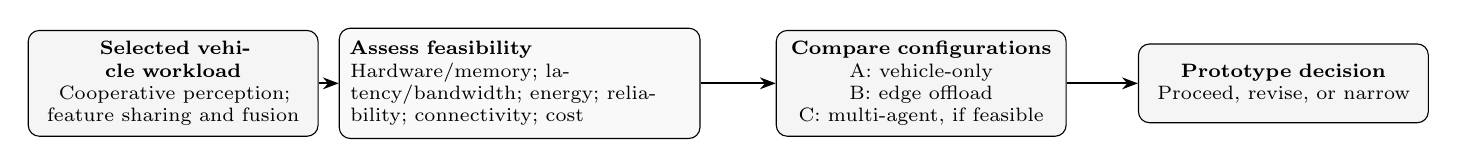
\begin{tikzpicture}[
      font=\scriptsize,
      block/.style={draw, rounded corners, fill=gray!8, align=center,
        text width=3.4cm, minimum height=1.0cm, inner sep=4pt},
      criteria/.style={draw, rounded corners, fill=gray!5, align=left,
        text width=4.3cm, minimum height=1.4cm, inner sep=4pt},
      flow/.style={-{Stealth[length=2mm]}, thick}
    ]
      \node[block] (select) at (0,0)
        {\textbf{Selected vehicle workload}\\Cooperative perception; feature sharing and fusion};
      \node[criteria] (assess) at (4.4,0)
        {\textbf{Assess feasibility}\\Hardware/memory; latency/bandwidth; energy; reliability; connectivity; cost};
      \node[block] (compare) at (9.5,0)
        {\textbf{Compare configurations}\\A: vehicle-only\\B: edge offload\\C: multi-agent, if feasible};
      \node[block] (decision) at (14.1,0)
        {\textbf{Prototype decision}\\Proceed, revise, or narrow};
      \draw[flow] (select.east) -- (assess.west);
      \draw[flow] (assess.east) -- (compare.west);
      \draw[flow] (compare.east) -- (decision.west);
    \end{tikzpicture}%
  }
  \caption{Proposed Feasibility-Assessment Framework.}
  \label{fig:feasibility-assessment-framework}
\end{figure}

\section{Proposed Technical Methodology}

\begin{samepage}
The primary technical direction is vehicle-to-vehicle and
vehicle-to-infrastructure cooperative perception. The ego vehicle performs
local inference and fuses selected information received from other agents.
The evaluation will consider:
\begin{enumerate}
  \item \textbf{Collaborative feature fusion:} exchange selected
  sensor-derived features or detection messages between agents and fuse
  them at the ego vehicle or a nearby edge node. Spatially selective
  communication is a candidate approach, not a finalized model choice
  \cite{v2xvit2022,where2comm2022,cobevt2023}.
  \item \textbf{Supporting edge offload:} assess whether an edge server
  should relay or process a selected non-safety-critical cooperative task.
  Compare the added compute capacity against transport delay, bandwidth,
  freshness, and interruption effects \cite{hou2022,v2xsurvey2025}.
  \item \textbf{Secondary training topic:} federated learning may be
  considered for later model improvement, but it is not part of the primary
  prototype unless time and resources permit
  \cite{flcav2024,mcmahan2017}.
\end{enumerate}

The initial CARLA prototype uses simulator ground-truth projections for
camera-label previews, a YOLO detector for object-detection timing, and a
PilotNet-style model for steering prediction from recorded autopilot data.
These components are separate experiments; they do not implement
cooperative perception. V2X payload, fusion location, edge participation,
and a suitable cooperative-perception model remain future design choices.
The team is entering the small-scale experimental phase and will document
available hardware, software, datasets, and network setup before assessing
those choices. Cooperative perception remains the intended primary online
workload, edge offloading a supporting comparison, and federated learning
a distinct, secondary training topic. Figure~\ref{fig:proposed-technical-paths}
distinguishes these roles.
\end{samepage}

\begin{figure}[H]
  \centering
  \resizebox{0.94\linewidth}{!}{%
    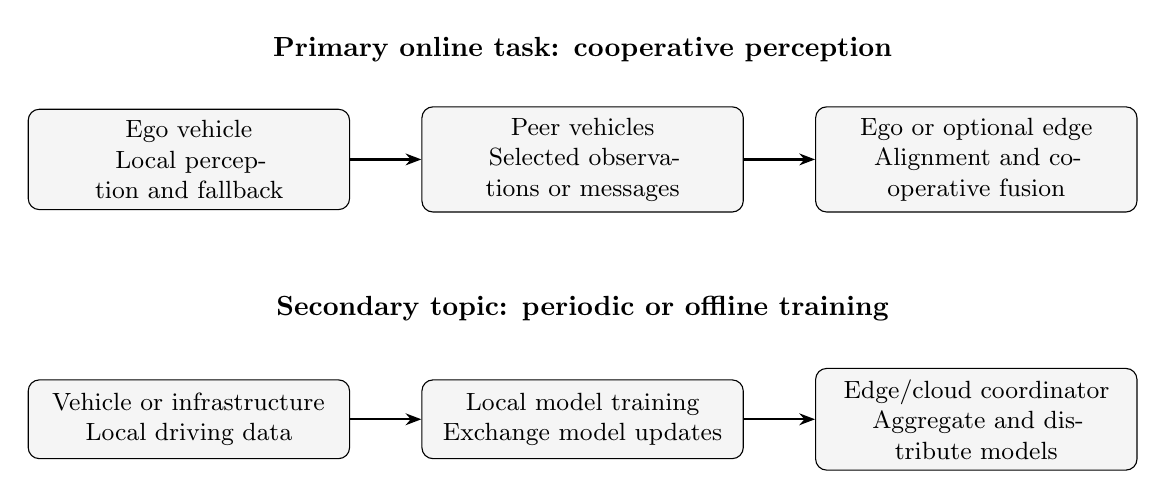
\begin{tikzpicture}[
      font=\small,
      block/.style={draw, rounded corners, fill=gray!8, align=center,
        text width=3.8cm, minimum height=1.0cm, inner sep=4pt},
      flow/.style={-{Stealth[length=2mm]}, thick}
    ]
      \node[font=\bfseries] at (0,3.4)
        {Primary online task: cooperative perception};
      \node[block] (sensor) at (-5.0,2.0)
        {Ego vehicle\\Local perception and fallback};
      \node[block] (agents) at (0,2.0)
        {Peer vehicles\\Selected observations or messages};
      \node[block] (fuse) at (5.0,2.0)
        {Ego or optional edge\\Alignment and cooperative fusion};
      \draw[flow] (sensor.east) -- (agents.west);
      \draw[flow] (agents.east) -- (fuse.west);
      \node[font=\bfseries] at (0,0.1)
        {Secondary topic: periodic or offline training};
      \node[block] (data) at (-5.0,-1.3)
        {Vehicle or infrastructure\\Local driving data};
      \node[block] (updates) at (0,-1.3)
        {Local model training\\Exchange model updates};
      \node[block] (aggregate) at (5.0,-1.3)
        {Edge/cloud coordinator\\Aggregate and distribute models};
      \draw[flow] (data.east) -- (updates.west);
      \draw[flow] (updates.east) -- (aggregate.west);
    \end{tikzpicture}%
  }
  \caption{Primary Cooperative Perception and Secondary Training Paths.}
  \label{fig:proposed-technical-paths}
\end{figure}

\section{Proposed System Architecture}

Each vehicle first processes its own camera, LiDAR, radar, and positioning
inputs through onboard preprocessing and local perception. An optional
feature-selection stage can prepare a message for V2V or V2I exchange:
raw observations preserve the most detail but can require high bandwidth;
intermediate features are model-dependent and trade representation size
against information; compact detections are smaller but less expressive.
Messages require pose and timestamp metadata so a receiving vehicle or
roadside node can align them and reject stale contributions
\cite{opv2v2022,where2comm2022,v2xsurvey2025}.

If feasible, a roadside edge server may relay information or host optional
alignment and cooperative fusion, returning only a sufficiently fresh
contribution. The ego vehicle combines usable remote information with its
own perception; if the link is unavailable or the contribution is late,
local perception continues without it. Cloud resources are reserved for
longer-term storage, offline training, and model management, not the live
safety-critical path. The diagram summarizes this proposal; its specific
model, message format, hardware, and task placement remain to be assessed.

\begin{figure}[H]
  \centering
  \resizebox{0.98\linewidth}{!}{%
    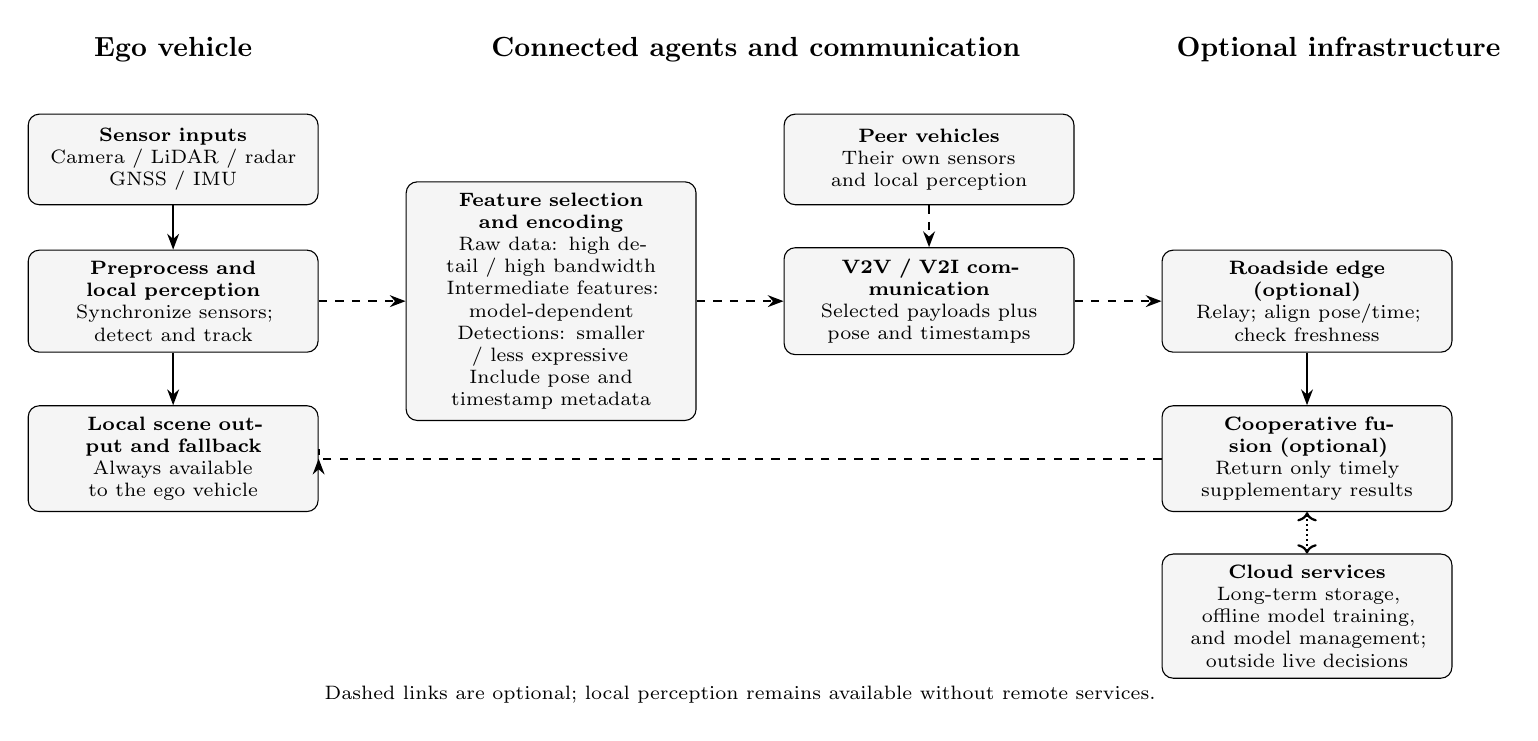
\begin{tikzpicture}[
      font=\scriptsize,
      block/.style={draw, rounded corners, fill=gray!8, align=center,
        text width=3.4cm, minimum height=1.15cm, inner sep=4pt},
      local/.style={-{Stealth[length=2mm]}, thick},
      optional/.style={-{Stealth[length=2mm]}, thick, dashed},
      support/.style={<->, densely dotted, thick}
    ]
      \node[font=\bfseries] at (0,5.4) {Ego vehicle};
      \node[font=\bfseries] at (7.4,5.4) {Connected agents and communication};
      \node[font=\bfseries] at (14.8,5.4) {Optional infrastructure};

      \node[block] (sensors) at (0,4.0)
        {\textbf{Sensor inputs}\\Camera / LiDAR / radar\\GNSS / IMU};
      \node[block] (localperception) at (0,2.2)
        {\textbf{Preprocess and local perception}\\Synchronize sensors; detect and track};
      \node[block] (localview) at (0,0.2)
        {\textbf{Local scene output and fallback}\\Always available to the ego vehicle};
      \node[block] (selector) at (4.8,2.2)
        {\textbf{Feature selection and encoding}\\
        Raw data: high detail / high bandwidth\\
        Intermediate features: model-dependent\\
        Detections: smaller / less expressive\\
        Include pose and timestamp metadata};
      \node[block] (peers) at (9.6,4.0)
        {\textbf{Peer vehicles}\\Their own sensors and local perception};
      \node[block] (v2x) at (9.6,2.2)
        {\textbf{V2V / V2I communication}\\Selected payloads plus pose and timestamps};
      \node[block] (align) at (14.4,2.2)
        {\textbf{Roadside edge (optional)}\\Relay; align pose/time; check freshness};
      \node[block] (fusion) at (14.4,0.2)
        {\textbf{Cooperative fusion (optional)}\\Return only timely supplementary results};
      \node[block] (cloud) at (14.4,-1.8)
        {\textbf{Cloud services}\\Long-term storage, offline model training,\\
        and model management; outside live decisions};

      \draw[local] (sensors.south) -- (localperception.north);
      \draw[local] (localperception.south) -- (localview.north);
      \draw[optional] (localperception.east) -- (selector.west);
      \draw[optional] (selector.east) -- (v2x.west);
      \draw[optional] (peers.south) -- (v2x.north);
      \draw[optional] (v2x.east) -- (align.west);
      \draw[local] (align.south) -- (fusion.north);
      \draw[optional] (fusion.west) -| (localview.east);
      \draw[support] (fusion.south) -- (cloud.north);
      \node[align=center] at (7.2,-2.8)
        {Dashed links are optional; local perception remains available without remote services.};
    \end{tikzpicture}%
  }
  \caption{Proposed Cooperative-Perception Architecture: Local Processing, V2X Payloads, Optional Edge Fusion, and Cloud Support.}
  \label{fig:proposed-av-architecture}
\end{figure}

\section{Proposed Experimental Setup}

The evaluation will compare configurations using the same input sequence,
model version, and output-quality measure:
\begin{enumerate}
  \item \textbf{Configuration A -- Vehicle-only:} one ego vehicle runs
  local perception using only its own sensor input. This is the baseline.
  \item \textbf{Configuration B -- Selected edge offload:} the ego vehicle
  sends a selected non-safety-critical processing task or payload to a
  roadside edge node. This isolates the effects of offloading and network
  conditions from multi-agent fusion.
  \item \textbf{Configuration C -- Multi-agent cooperative perception:}
  the ego vehicle receives and fuses sensor-derived information from other
  vehicles or infrastructure. The fusion location and payload type remain
  open design choices.
\end{enumerate}

OPV2V is a candidate dataset: it provides simulated V2V scenes, LiDAR data,
annotations, and baseline fusion strategies generated with CARLA and
OpenCDA \cite{opv2v2022}. Its format, access, licensing, model compatibility,
and computational requirements must be checked against available resources
before configuration C is committed. If multi-agent data or compute are
not feasible, A and B remain the bounded evaluation; configuration C is
not promised as a completed prototype. Any simulation-based results would
also require a clear caveat about transfer to real vehicles.

The specific boards, servers, software stack, and model will be selected
after the team inventories available resources. The test record will
include hardware and software versions, model configuration, input
resolution and sequence, warm-up procedure, repeated-run protocol, and
network conditions. A controlled vehicle--edge link will vary measured
latency, available bandwidth, and interruption conditions; an offline run
will verify local fallback. No safety-critical output depends on edge or
cloud service.

All applicable configurations will use the metrics in
Table~\ref{tab:proposed-evaluation-metrics}; A and B are the initial
comparison, while C is conditional on confirming the multi-agent resource
requirements. No live-road safety claim is made. Figure~\ref{fig:experimental-workflow}
summarises the proposed comparison; network profiles and acceptance
thresholds remain to be established from the selected workload and setup.

\begin{figure}[H]
  \centering
  \resizebox{0.98\linewidth}{!}{%
    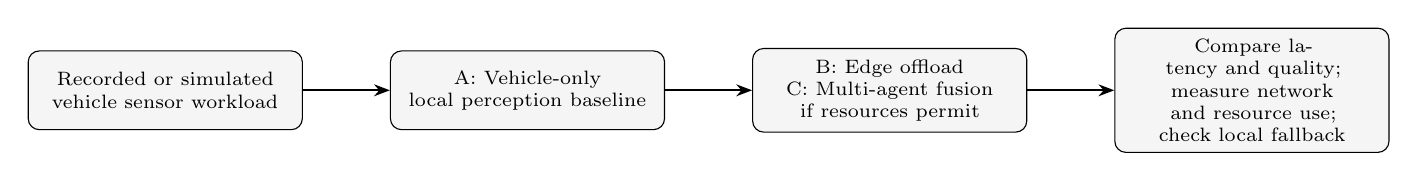
\begin{tikzpicture}[
      font=\scriptsize,
      stage/.style={draw, rounded corners, fill=gray!8, align=center,
        text width=3.2cm, minimum height=1.0cm, inner sep=4pt},
      flow/.style={-{Stealth[length=2mm]}, thick}
    ]
      \node[stage] (input) at (0,0)
        {Recorded or simulated\\vehicle sensor workload};
      \node[stage] (baseline) at (4.6,0)
        {A: Vehicle-only\\local perception baseline};
      \node[stage] (distributed) at (9.2,0)
        {B: Edge offload\\C: Multi-agent fusion\\if resources permit};
      \node[stage] (compare) at (13.8,0)
        {Compare latency and quality;\\measure network and resource use;\\check local fallback};
      \draw[flow] (input.east) -- (baseline.west);
      \draw[flow] (baseline.east) -- (distributed.west);
      \draw[flow] (distributed.east) -- (compare.west);
    \end{tikzpicture}%
  }
  \caption{Proposed Experimental Evaluation Workflow.}
  \label{fig:experimental-workflow}
\end{figure}

\section{Performance Evaluation Metrics}

The metrics below guide the ongoing small-scale experiments and the planned
cooperative evaluation. Initial detector latency results are reported in
Section~\ref{subsec:carla-results}; cooperative network and multi-agent
metrics remain future work. Each run should use consistent timing
boundaries and record the workload, hardware, software, and network
configuration. Detection-quality metrics apply when the chosen model and
annotated data support them.

\begin{table}[H]
  \centering
  \footnotesize
  \renewcommand{\arraystretch}{1.15}
  \caption{Proposed Performance Evaluation Metrics.}
  \label{tab:proposed-evaluation-metrics}
  \begin{tabularx}{\textwidth}{
    >{\raggedright\arraybackslash}p{0.24\textwidth}
    >{\raggedright\arraybackslash}X}
    \toprule
    Evaluation parameter & Proposed measurement \\
    \midrule
    Inference latency & Time from model input being available to the corresponding inference output. \\
    End-to-end latency & Time from sensor sample or frame input to the system's perception output, including preprocessing and any communication. \\
    Detection quality & Precision, recall, and/or mean average precision (mAP), as supported by the selected task and annotated data. \\
    Throughput & Processed frames or samples per second under a stated workload and configuration. \\
    Network latency & Measured one-way or round-trip delay for vehicle--edge communication, with the measurement definition stated. \\
    Bandwidth usage & Bytes transferred per sample or time interval, reported separately for inputs, intermediate data, and outputs where possible. \\
    Energy consumption & Energy used during a defined processing interval, measured with suitable instrumentation when available. \\
    Resource utilization & CPU, GPU or accelerator, and memory utilization on vehicle and edge nodes during each run. \\
    Message freshness & Age of the received timestamped input or result at fusion time; stale contributions are excluded. \\
    Network reliability & Packet loss and interruption duration observed during the stated test profile. \\
    \bottomrule
  \end{tabularx}
\end{table}

\chapter{Results and Discussion}

\noindent
This chapter combines literature findings with preliminary CARLA
measurements. The simulator results describe only the tested perception and
steering pipeline; they do not measure V2V cooperation or validate a road
vehicle.

\section{Literature Synthesis}

The reviewed literature converges on layered end-edge-cloud architectures,
with federated training and partitioned or collaborative inference as two
major technical families \cite{deng2020,hou2022}. Communication efficiency
is a recurring bottleneck across both. For the selected autonomous-vehicle
application, the central question is how communication-enabled
multi-agent perception can improve environmental awareness without relying
on remote connectivity for immediate decisions. Table~\ref{tab:literature-comparison}
compares the selected studies by problem, technique, workload, evaluation
context, limitations, and relevance. Numerical findings are source-specific
and are not directly comparable because datasets, hardware, network
assumptions, and metrics differ. The cited works motivate the proposal but
do not establish the performance of the proposed system.

\begingroup
\footnotesize
\setlength{\tabcolsep}{3pt}
\renewcommand{\arraystretch}{1.18}
\begin{longtable}{
  >{\raggedright\arraybackslash}p{0.135\textwidth}
  >{\raggedright\arraybackslash}p{0.275\textwidth}
  >{\raggedright\arraybackslash}p{0.265\textwidth}
  >{\raggedright\arraybackslash}p{0.265\textwidth}}
\caption{Comparison of reviewed methods, evaluation contexts, limitations, and project relevance.}
\label{tab:literature-comparison}\\
\toprule
Study & Problem and proposed technique & Evaluation setting and evidence & Limitations and project relevance \\
\midrule
\endfirsthead
\caption[]{Comparison of reviewed methods and evidence (continued).}\\
\toprule
Study & Problem and proposed technique & Evaluation setting and evidence & Limitations and project relevance \\
\midrule
\endhead
\midrule
\multicolumn{4}{r}{Continued on next page}\\
\endfoot
\bottomrule
\endlastfoot

\textbf{Hu et al. (2023)} \cite{hu2023} &
Dynamic placement of a containerized video object-detection pipeline across heterogeneous edge devices. &
Raspberry Pi, MacBook Pro, and Asus nodes in Kubernetes; varies video quality and detector count and measures frame-processing time. &
\textbf{Limitations:} One video workload and deployment; additional containers eventually increase processing time. \par\smallskip
\textbf{Relevance:} Motivates measuring coordination and communication cost instead of assuming more edge nodes always help. \\
\addlinespace
\textbf{Deng et al. (2020)} \cite{deng2020} &
Taxonomy of AI for edge and AI on edge; surveys architecture, training, inference, and challenges. &
Literature synthesis; no single dataset, hardware setup, or benchmark metric. &
\textbf{Limitations:} Survey scope and definitions vary; not experimental evidence for a vehicle system. \par\smallskip
\textbf{Relevance:} Provides terminology for classifying vehicle, edge, and cloud roles. \\
\addlinespace
\textbf{Hou et al. (2022)} \cite{hou2022} &
DistrEdge uses deep reinforcement learning to partition CNN inference across heterogeneous edge devices. &
Jetson devices and varying Wi-Fi bandwidth; reports latency, throughput, and speedup against tested baselines. &
\textbf{Limitations:} Memory constraints are not modeled; results depend on tested models, devices, and networks. \par\smallskip
\textbf{Relevance:} Supports edge offload as a secondary comparison and motivates measuring communication and memory costs. \\
\addlinespace
\textbf{McMahan et al. (2017)} \cite{mcmahan2017} &
Federated averaging aggregates locally computed model updates for decentralized training. &
Five architectures and four datasets; compares communication rounds with synchronized SGD. &
\textbf{Limitations:} Training-focused, not an inference or cooperative-perception evaluation; results depend on workload and data partition. \par\smallskip
\textbf{Relevance:} Background for the secondary federated-training topic, not the primary prototype. \\
\addlinespace
\textbf{Biswas and Wang (2023)} \cite{biswas2023} &
Reviews integration of IoT, edge intelligence, 5G, and blockchain in autonomous-vehicle systems. &
Literature review; no single experimental setup or performance metric. &
\textbf{Limitations:} Review evidence rather than a common prototype benchmark. \par\smallskip
\textbf{Relevance:} Provides application context and discusses safety, security, and reliability needs. \\
\addlinespace
\textbf{Chellapandi et al. (2024)} \cite{flcav2024} &
Surveys centralized and decentralized federated learning for connected and automated vehicles, including privacy and security techniques. &
Reviews published applications, models, and datasets; no new common experimental benchmark. &
\textbf{Limitations:} Survey-level evidence; communication, heterogeneity, and security remain open challenges. \par\smallskip
\textbf{Relevance:} Supports the secondary training direction and distinguishes it from online perception. \\
\addlinespace
\textbf{Xu et al. (2022), V2X-ViT} \cite{v2xvit2022} &
Heterogeneous multi-agent and multi-scale window attention fuses V2X information for LiDAR 3D detection. &
CARLA/OpenCDA simulation with V2X-Sim; reports a 21.2\% AP gain over single-agent and at least 7.3\% over compared intermediate-fusion baselines. &
\textbf{Limitations:} Simulation-to-reality generalization and scalability; privacy and adversarial robustness also remain concerns. \par\smallskip
\textbf{Relevance:} Supports cooperative fusion and testing pose, timing, heterogeneity, and communication constraints. \\
\addlinespace
\textbf{Hu et al. (2022)}\par\textit{Where2comm} \cite{where2comm2022} &
Spatial confidence maps select sparse, perceptually important feature regions and adapt shared regions to bandwidth. &
Camera/LiDAR vehicle and drone scenarios across OPV2V, V2X-Sim, DAIR-V2X, and CoPerception-UAVs; measures AP and communication bytes. &
\textbf{Limitations:} Benchmark-specific results; does not establish temporal scheduling or real wireless deployment. \par\smallskip
\textbf{Relevance:} Informs communication-aware sharing and joint measurement of bytes, latency, and detection quality. Reported communication reductions (including over $100{,}000\times$ in selected OPV2V comparisons) are protocol-specific. \\
\addlinespace
\textbf{Xu et al. (2022), OPV2V} \cite{opv2v2022} &
Open simulated V2V dataset and benchmark for early, late, and intermediate LiDAR fusion, including Attentive Intermediate Fusion. &
CARLA/OpenCDA; 73 scenes, 11,464 frames, and 232,913 annotated 3D vehicle boxes; evaluates fusion strategies. &
\textbf{Limitations:} Simulation does not establish transfer to real traffic or real V2V networks. \par\smallskip
\textbf{Relevance:} Candidate dataset for configuration C, subject to resource, licensing, and format checks. \\
\addlinespace
\textbf{Xu et al. (2023), CoBEVT} \cite{cobevt2023} &
Sparse fused axial attention combines multi-view, multi-agent camera features for cooperative bird's-eye-view segmentation. &
PMLR conference paper; evaluates BEV segmentation on OPV2V and reports extensions to single-agent multi-camera segmentation and multi-agent LiDAR 3D detection, including inference speed. &
\textbf{Limitations:} Dataset-based evaluation does not establish performance over a deployed vehicle communication stack. \par\smallskip
\textbf{Relevance:} Offers an alternative fusion model and candidate segmentation or detection tasks. \\
\addlinespace
\textbf{Huang et al. (2025)} \cite{v2xsurvey2025} &
Survey of V2X cooperative-perception models, collaboration strategies, agent selection, alignment, and fusion. &
Literature synthesis; no new common benchmark. &
 \textbf{Limitations:} Identifies delay, data loss, heterogeneous agents/models, and uncertain perception as unresolved challenges. \par\smallskip
\textbf{Relevance:} Supports network-interruption, alignment, freshness, and heterogeneity criteria in the proposed evaluation. \\
\end{longtable}
\endgroup

The vehicle-specific papers address complementary parts of the proposed
problem: V2X-ViT and CoBEVT study fusion architectures, Where2comm targets
communication cost, OPV2V supplies a simulated V2V benchmark, and the
cooperative-perception survey summarizes system-level challenges
\cite{v2xvit2022,where2comm2022,opv2v2022,cobevt2023,v2xsurvey2025}.
The federated-learning survey instead concerns model training
\cite{flcav2024}. The reported AP, communication, and timing measures use
different datasets, hardware, and protocols and must not be ranked as if
they came from a common experiment.

\section{Feasibility Indications}

The reviewed cooperative-perception studies establish feasible research
baselines for multi-agent fusion on simulated datasets, and Where2comm
provides a concrete method for trading communication volume against
perception quality \cite{v2xvit2022,where2comm2022,cobevt2023}. OPV2V is a
candidate dataset for an initial evaluation, but its simulated scenes do
not establish real-road performance \cite{opv2v2022}. The evidence therefore
supports a bounded prototype study, not a claim that the proposed system
meets deployment or safety requirements. Hu et al.\ report diminishing
returns from adding detection containers in their video pipeline, while
Hou et al.\ report 1.1--3$\times$ speedup only against the baselines in
their own distributed CNN-inference evaluation \cite{hu2023,hou2022}.
These results use different workloads and test settings and are not
directly comparable.

\subsection{Initial CARLA Prototype Results}
\label{subsec:carla-results}

Our initial small-scale CARLA experiments have produced the following
findings. These are simulator measurements from our project, not results
from the cited cooperative-perception papers.

\begin{itemize}
  \item \textbf{Ground-truth label projection:} \texttt{make\_labels.py}
  projected CARLA ground-truth object boxes into camera images in clear,
  rain, fog, and night conditions. These boxes are simulator labels, not
  YOLO predictions.
  \item \textbf{Driving-data capture:} \texttt{record\_drive.py} recorded
  synchronized left, center, and right camera images. The side cameras are
  only 0.5\,m off-center and can provide nearly duplicate views, limiting
  the diversity of this setup.
  \item \textbf{Detector timing:} \texttt{detect.py} was benchmarked for
  198 frames per configuration. Mean end-to-end/model-only latency was
  45.1/33.8\,ms on CPU FP32, 20.5/9.8\,ms on GPU FP32, and 20.3/10.1\,ms on
  GPU FP16. GPU FP32 end-to-end p95 was 24.2\,ms. A separate clean rerender
  of 600 GPU FP32 frames averaged 20.9\,ms with 23.2\,ms p95. The rerender
  is a distinct test, not additional samples from the detector benchmark.
  The CPU end-to-end mean is above the 33.3\,ms frame-time reference for
  30 FPS, while the two GPU means are below it; this does not establish
  real-time vehicle performance.
  \item \textbf{Steering-model training:} Two 25-epoch runs trained a
  PilotNet-style model on CARLA autopilot data with 450 validation samples.
  Run 2 (seed 0) is the primary saved run. Its validation MAE was lowest at
  epoch 1 and did not improve thereafter; final epoch-25 overall MAE was
  0.0863. At epoch 25, MAE was 0.0471 on 303 straight samples, 0.0616 on
  35 mild samples, and 0.2004 on 112 turn samples. The always-straight
  baseline scored 0.0023, 0.0433, and 0.1576 on those same groups,
  respectively. Overall, the baseline MAE was 0.0441, compared with 0.0512
  at the saved epoch-1 checkpoint and 0.0863 at epoch 25. On turns, these
  MAEs were 0.1576, 0.1660, and 0.2004. Turn direction matched the target
  in 49\% of cases. The saved model therefore did not beat the simple
  baseline. Run 1 was unseeded and is reported separately: its overall
  validation MAE changed from 0.0589 at epoch 1 to 0.0773 at epoch 25, and
  its turns-only MAE changed from 0.1686 to 0.1922. The two runs should not
  be pooled.
\end{itemize}

The following figures present our preliminary CARLA findings. The
ground-truth projection examples are simulator labels, not detector predictions. The
detector benchmark shows the CPU end-to-end mean above, and the GPU means
below, the 30 FPS frame-time reference in this particular setup. The
steering model did not outperform the
always-straight baseline; its lowest validation MAE occurred at epoch 1,
consistent with overfitting in later epochs. Our experiment records do not
yet specify the CARLA version, GPU model, detector weights/architecture, or
validation-data collection conditions. We should document these details
before attempting a reproducible comparison. No steering result is a
safety claim.

\begin{figure}[H]
  \centering
  \begin{minipage}[t]{0.48\textwidth}
    \centering
    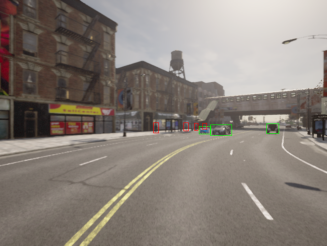
\includegraphics[width=0.96\linewidth]{images/carla_ground_truth_clear.png}\\
    \small Clear weather
  \end{minipage}\hfill
  \begin{minipage}[t]{0.48\textwidth}
    \centering
    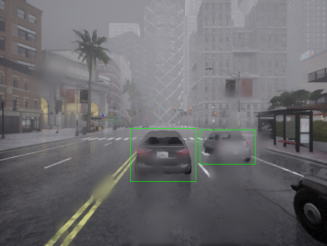
\includegraphics[width=0.96\linewidth]{images/carla_ground_truth_rain.png}\\
    \small Rain weather
  \end{minipage}

  \vspace{0.4em}
  \begin{minipage}[t]{0.48\textwidth}
    \centering
    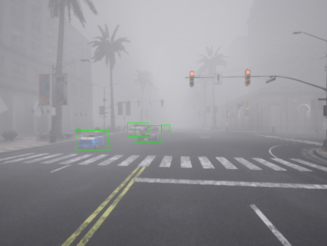
\includegraphics[width=0.96\linewidth]{images/carla_ground_truth_fog.png}\\
    \small Fog weather
  \end{minipage}\hfill
  \begin{minipage}[t]{0.48\textwidth}
    \centering
    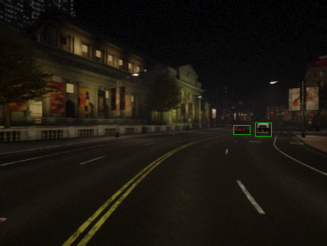
\includegraphics[width=0.96\linewidth]{images/carla_ground_truth_night.png}\\
    \small Night weather
  \end{minipage}
  \caption{CARLA ground-truth vehicle and pedestrian boxes projected into
  camera images under four weather conditions. These are labels generated
  by \texttt{make\_labels.py}, not YOLO detections. Source: our CARLA
  ground-truth projections.}
  \label{fig:carla-weather-labels}
\end{figure}

\begin{figure}[H]
  \centering
  \begin{minipage}[t]{0.48\textwidth}
    \centering
    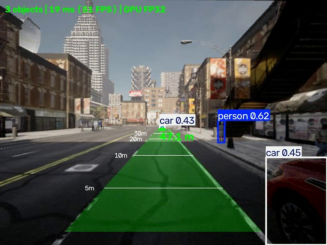
\includegraphics[width=\linewidth]{images/carla_demo_frame_0001.png}\\
    \small Clip at 00:01
  \end{minipage}\hfill
  \begin{minipage}[t]{0.48\textwidth}
    \centering
    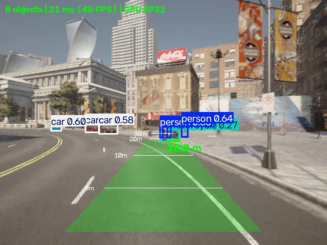
\includegraphics[width=\linewidth]{images/carla_demo_frame_0009.png}\\
    \small Clip at 00:09
  \end{minipage}
  \caption{Annotated CARLA demo frames from a separate 600-frame GPU FP32
  rerender (mean 20.9\,ms, p95 23.2\,ms). HUD values shown are individual
  frames. Source: our CARLA demo rerender.}
  \label{fig:carla-demo-frames}
\end{figure}

\begin{figure}[H]
  \centering
  \begin{minipage}[t]{0.32\textwidth}
    \centering
    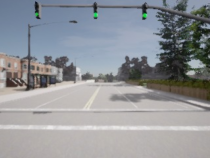
\includegraphics[width=\linewidth]{images/carla_drive_left.png}\\
    \small Left camera
  \end{minipage}\hfill
  \begin{minipage}[t]{0.32\textwidth}
    \centering
    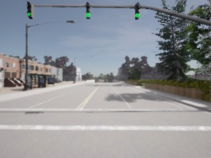
\includegraphics[width=\linewidth]{images/carla_drive_center.png}\\
    \small Center camera
  \end{minipage}\hfill
  \begin{minipage}[t]{0.32\textwidth}
    \centering
    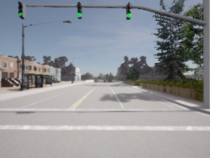
\includegraphics[width=\linewidth]{images/carla_drive_right.png}\\
    \small Right camera
  \end{minipage}
  \caption[Synchronized three-camera CARLA capture]{Synchronized camera
  triplet for frame 0170518. The side cameras
  are only 0.5\,m off-center, so their views can be nearly identical.
  Source: our saved \texttt{drive\_data/img} samples, recorded by
  \texttt{record\_drive.py}.}
  \label{fig:carla-camera-triplet}
\end{figure}

\begin{figure}[H]
  \centering
  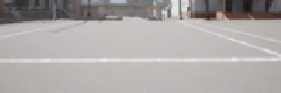
\includegraphics[width=0.46\textwidth]{images/carla_steering_input.png}
  \caption{PilotNet-style model input crop (200 by 66 pixels), enlarged for
  display. Source: our CARLA training data and preprocessing.}
  \label{fig:carla-steering-input}
\end{figure}

\begin{figure}[H]
  \centering
  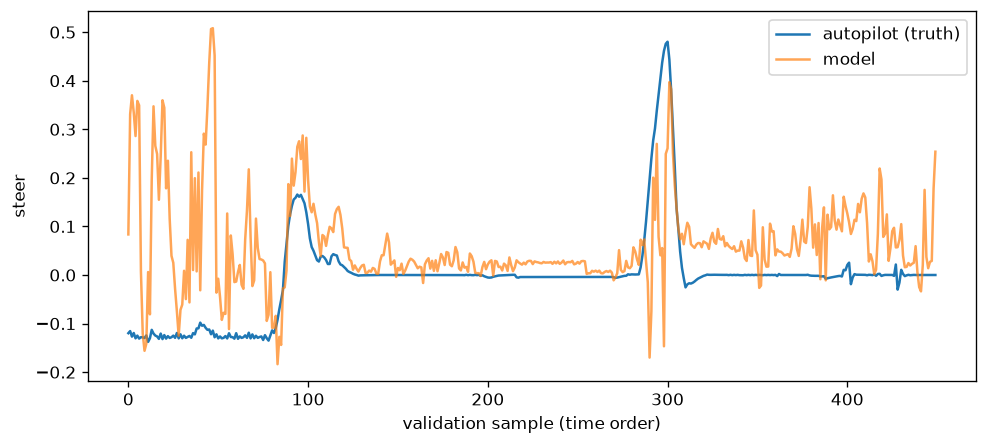
\includegraphics[width=0.90\textwidth]{images/carla_steering_val_pred_sequence.png}
  \par\smallskip
  \small\textbf{(a)} Steering values across validation samples: autopilot
  labels and model predictions.

  \medskip
  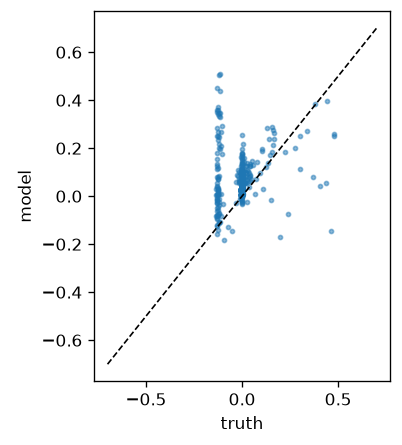
\includegraphics[width=0.43\textwidth]{images/carla_steering_val_pred_scatter.png}
  \par\smallskip
  \small\textbf{(b)} Predicted steering versus target; the dashed line is
  equality.
  \caption[Run 2 final-epoch validation diagnostics]{Run 2 final-epoch
  validation predictions. The two panels are shown separately at readable
  sizes with their aspect ratios preserved. This diagnostic does not
  establish a reliable driving policy. Source: our validation run,
  \texttt{results/val\_pred.png}.}
  \label{fig:carla-steering-validation}
\end{figure}

\begin{figure}[H]
  \centering
  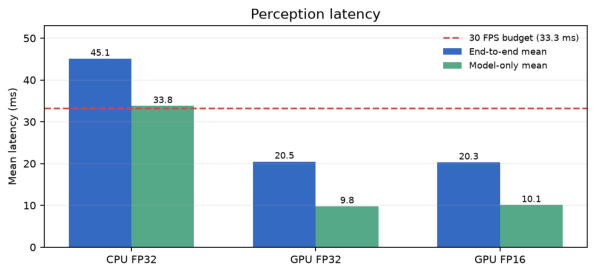
\includegraphics[width=0.88\textwidth]{images/carla_detector_latency.png}
  \caption{Mean model-only and end-to-end detector latency for 198 frames
  per configuration. The dashed line marks the 33.3\,ms frame-time
  reference for 30 FPS. CPU FP32 end-to-end mean exceeds the reference;
  GPU FP32 and FP16 means are below it. Source: \texttt{detect.py} and the
  baseline CSV files from our timing tests.}
  \label{fig:carla-detector-latency}
\end{figure}

\begin{figure}[H]
  \centering
  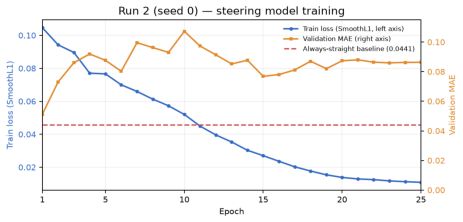
\includegraphics[width=0.78\textwidth]{images/carla_run2_training_curve.png}
  \caption[Run 2 steering loss and validation MAE]{Run 2 (seed 0)
  steering-model training loss and validation MAE.
  The lowest validation MAE occurs at epoch 1 and does not improve
  afterward, although training loss continues to fall. The axes show
  different metrics; line crossings have no meaning. Source:
  our \texttt{results/steer\_training\_curve.csv}.}
  \label{fig:carla-run2-training}
\end{figure}

\begin{figure}[H]
  \centering
  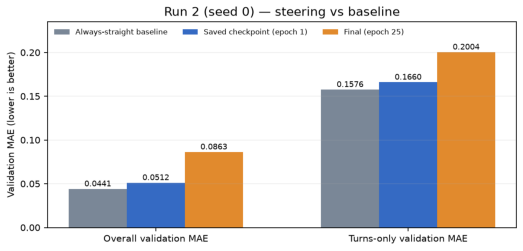
\includegraphics[width=0.82\textwidth]{images/carla_run2_vs_baseline.png}
  \caption{Run 2 (seed 0): always-straight baseline, saved epoch-1
  checkpoint, and epoch-25 steering model. Lower MAE is better; the trained
  model does not beat the baseline overall or on turns. Source: our Run 2
  terminal log and training CSV.}
  \label{fig:carla-run2-baseline}
\end{figure}

\subsection{Research Gaps Identified}

The following open issues recur in the reviewed cooperative-perception
literature; they are established research challenges, not original
discoveries of this project:
\begin{enumerate}
  \item \textbf{Communication overhead:} exchanging full observations or
  dense features can compete with available V2X bandwidth. Where2comm
  explores spatially selective feature sharing, but its reported
  communication gains are tied to the evaluated datasets and protocols
  \cite{where2comm2022,opv2v2022}.
  \item \textbf{Latency and freshness:} transmission, feature processing,
  pose alignment, and fusion contribute to end-to-end delay; information
  that arrives late may no longer be useful. The survey identifies
  transmission delay and data loss as ongoing V2X challenges
  \cite{v2xsurvey2025}.
  \item \textbf{Intermittent connectivity:} mobility, packet loss, and
  variable link conditions can interrupt or degrade cooperative inputs.
  Published benchmark results do not by themselves establish reliability
  over a real vehicle-to-edge wireless link \cite{v2xsurvey2025,opv2v2022}.
  \item \textbf{Agent and hardware heterogeneity:} differences in sensors,
  models, pose estimates, and compute capability complicate information
  alignment and fusion \cite{v2xvit2022,v2xsurvey2025}.
  \item \textbf{Local fallback:} cooperative-perception methods augment a
  vehicle's view, but a vehicle still needs local perception when remote
  messages are absent or stale. This requirement shapes our architecture
  and offline test; it is not evidence that the cited models alone provide
  a safety guarantee.
\end{enumerate}

Table~\ref{tab:av-workload-allocation} gives an illustrative allocation
for further analysis. It is a proposed starting point, not a measured or
final task-placement policy. The final placement should be justified
against the reviewed evidence, selected workload, and feasibility results.

\begin{table}[H]
  \centering
  \footnotesize
  \renewcommand{\arraystretch}{1.15}
  \caption{Illustrative Mapping of Autonomous-Vehicle Workloads to Computing Layers.}
  \label{tab:av-workload-allocation}
  \begin{tabularx}{\textwidth}{
    >{\raggedright\arraybackslash}p{0.32\textwidth}
    >{\centering\arraybackslash}p{0.17\textwidth}
    >{\centering\arraybackslash}p{0.17\textwidth}
    >{\centering\arraybackslash}X}
    \toprule
    Workload & Vehicle & Edge & Cloud \\
    \midrule
    Sensor acquisition & Primary & -- & -- \\
    Local perception and fallback & Primary & -- & -- \\
    Cooperative messages (features/detections) & Primary & Relay possible & -- \\
    Cooperative fusion & Primary or edge & Optional & -- \\
    Federated model training (secondary) & Possible & Possible & Primary coordinator \\
    Model management & -- & Distribution relay & Primary \\
    \bottomrule
  \end{tabularx}
\end{table}

\section{Discussion and Limitations}

The synthesis indicates a trade-off between latency and energy on one side
and communication cost on the other. Moving computation closer to the data
may reduce latency and bandwidth pressure, but lower edge computing
capacity and device heterogeneity can require model partitioning,
compression, or collaborative execution. Non-IID data and
slow or unreliable nodes can create stragglers and dropouts.
Privacy and security risks, including inference and poisoning attacks, also
constrain how data and model updates are handled.

For autonomous vehicles, communication interruptions can make an offloaded
result late or unavailable, and vehicle mobility can make edge access
intermittent. Onboard compute, memory, power, and thermal limits constrain
local models, while added edge or cloud processing can increase network
load and create freshness or coordination problems. Cooperative perception
also raises questions about sensor alignment, data authenticity, and the
privacy of location and scene information. The architecture therefore
retains a local processing path and treats remote contributions as
supplementary; the safety and reliability of any future implementation
would require separate validation beyond the performance metrics proposed
here.

Initial implementation and measurements have been carried out in CARLA, but
they cover only the camera-label, detector-latency, and steering experiments
described above. They do not measure cooperative V2V/V2I communication,
distributed inference, edge offloading, or multi-agent perception quality.
The detector timings are specific to their hardware, model, and test
procedure; literature results and separate benchmarks should not be
compared as if measured in a common setup. The steering model's failure to
outperform the always-straight baseline is an important limitation, not
evidence of autonomous-driving capability. The field is still developing,
and open challenges include resource constraints, security threats,
scalability, and communication overhead.

\section{Additional Sources and Evidence}

The following two papers were added to the source collection after the
eleven-work core review described in the Review Protocol. They extend that
discussion without changing the project's scope.

The newly added CoEdge study examines cooperative execution of a single
deep neural network across heterogeneous edge devices. Its adaptive
partitioning responds to device capability and network conditions. In a
prototype evaluation with four CNN models, the authors report energy
reductions of 25.5--66.9\% with close inference latency relative to the
compared approaches \cite{coedge2021}. These results motivate measuring
energy alongside latency and communication cost when resources permit, but
they are specific to the study's models, devices, and network conditions.
They do not establish the same gains for a vehicle deployment.

This form of cooperation differs from multi-agent cooperative perception:
CoEdge distributes the computation for a model across devices, whereas
vehicle-to-vehicle perception combines information from distinct agents.
Both involve communication between nodes, but address different workload
and perception objectives. Figure~\ref{fig:coedge-inference} gives an
original conceptual view of the former, based on the approach described by
Zeng et al.\ \cite{coedge2021}.

\begin{figure}[H]
  \centering
  \resizebox{0.98\linewidth}{!}{%
    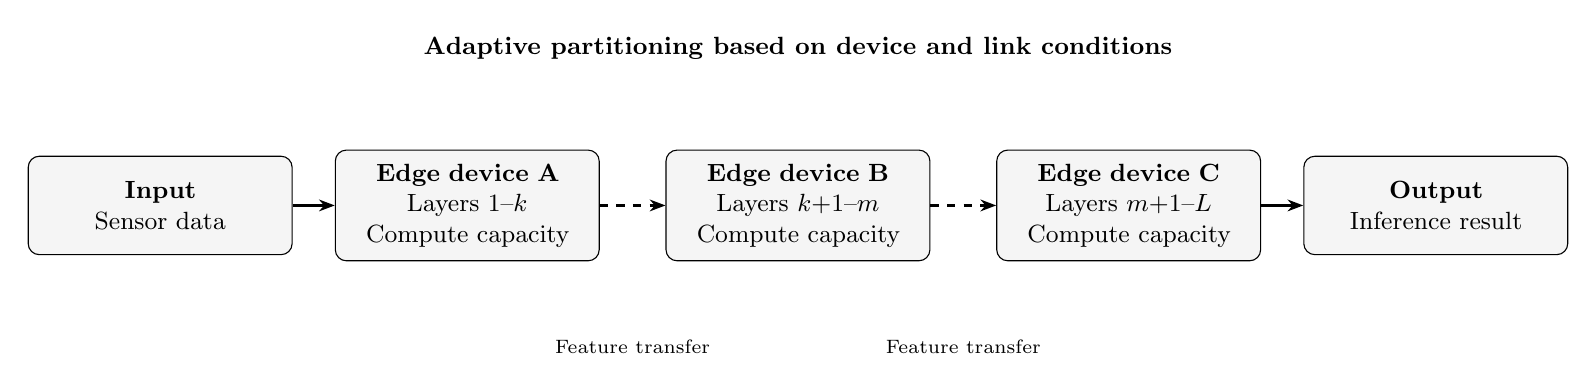
\begin{tikzpicture}[
      font=\small,
      device/.style={draw, rounded corners, fill=gray!8, align=center,
        text width=3.0cm, minimum height=1.25cm, inner sep=5pt},
      flow/.style={-{Stealth[length=2mm]}, thick},
      transfer/.style={-{Stealth[length=2mm]}, thick, dashed}
    ]
      \node[device] (input) at (-3.4,0)
        {\textbf{Input}\\Sensor data};
      \node[device] (nodea) at (0.5,0)
        {\textbf{Edge device A}\\Layers 1--$k$\\Compute capacity};
      \node[device] (nodeb) at (4.7,0)
        {\textbf{Edge device B}\\Layers $k{+}1$--$m$\\Compute capacity};
      \node[device] (nodec) at (8.9,0)
        {\textbf{Edge device C}\\Layers $m{+}1$--$L$\\Compute capacity};
      \node[device] (output) at (12.8,0)
        {\textbf{Output}\\Inference result};
      \draw[flow] (input.east) -- (nodea.west);
      \draw[transfer] (nodea.east) -- (nodeb.west);
      \draw[transfer] (nodeb.east) -- (nodec.west);
      \draw[flow] (nodec.east) -- (output.west);
      \node[align=center] at (4.7,2.0)
        {\textbf{Adaptive partitioning based on device and link conditions}};
      \node[font=\scriptsize,fill=white,inner sep=1pt] at (2.6,-1.8)
        {Feature transfer};
      \node[font=\scriptsize,fill=white,inner sep=1pt] at (6.8,-1.8)
        {Feature transfer};
    \end{tikzpicture}%
  }
  \caption[Cooperative DNN Inference across Heterogeneous Edge Devices]{
    Conceptual view of cooperative DNN inference across heterogeneous edge
    devices. Original schematic based on Zeng et al.\ \cite{coedge2021};
    it is not reproduced from the source paper.}
  \label{fig:coedge-inference}
\end{figure}

The relative energy savings reported for CoEdge's four evaluated CNNs are
summarized in Figure~\ref{fig:coedge-energy-saving}. The values come from
the paper's comparison with local inference and Musical Chair; they are
study-specific results, not measurements from this project
\cite{coedge2021}.

\begin{figure}[H]
  \centering
  \resizebox{0.95\linewidth}{!}{%
    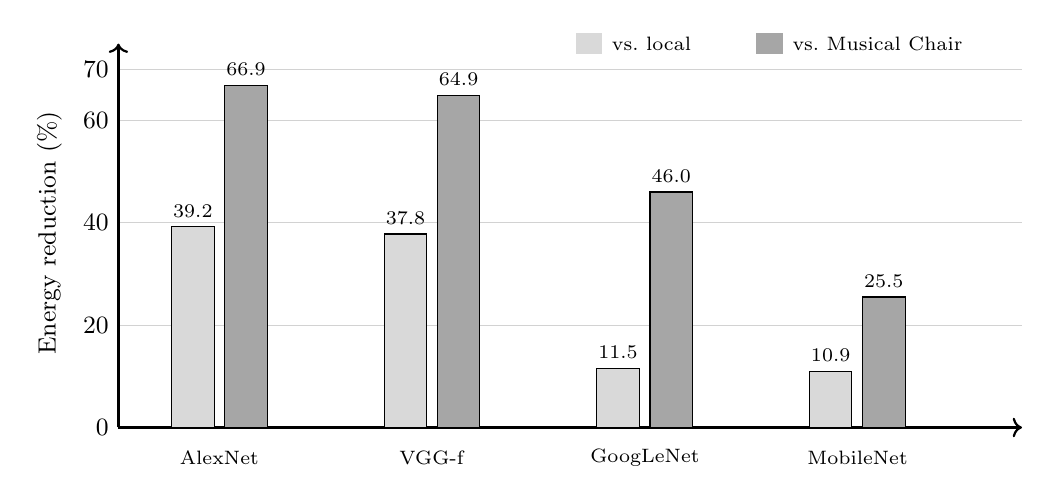
\begin{tikzpicture}[
      x=1.35cm,
      y=0.065cm,
      localbar/.style={draw=black, fill=gray!30},
      cooperativebar/.style={draw=black, fill=gray!70},
      font=\small
    ]
      \foreach \y in {0,20,40,60,70} {
        \draw[gray!35] (0,\y) -- (8.5,\y);
        \node[left] at (0,\y) {\y};
      }
      \draw[thick,->] (0,0) -- (0,75);
      \draw[thick,->] (0,0) -- (8.5,0);
      \node[rotate=90] at (-0.65,38) {Energy reduction (\%)};

      \fill[localbar] (0.5,0) rectangle (0.9,39.2);
      \node[above,font=\scriptsize] at (0.7,39.2) {39.2};
      \fill[cooperativebar] (1.0,0) rectangle (1.4,66.9);
      \node[above,font=\scriptsize] at (1.2,66.9) {66.9};
      \node[font=\scriptsize,align=center,text width=1.8cm] at (0.95,-6)
        {AlexNet};

      \fill[localbar] (2.5,0) rectangle (2.9,37.8);
      \node[above,font=\scriptsize] at (2.7,37.8) {37.8};
      \fill[cooperativebar] (3.0,0) rectangle (3.4,64.9);
      \node[above,font=\scriptsize] at (3.2,64.9) {64.9};
      \node[font=\scriptsize,align=center,text width=1.8cm] at (2.95,-6)
        {VGG-f};

      \fill[localbar] (4.5,0) rectangle (4.9,11.5);
      \node[above,font=\scriptsize] at (4.7,11.5) {11.5};
      \fill[cooperativebar] (5.0,0) rectangle (5.4,46.0);
      \node[above,font=\scriptsize] at (5.2,46.0) {46.0};
      \node[font=\scriptsize,align=center,text width=1.8cm] at (4.95,-6)
        {GoogLeNet};

      \fill[localbar] (6.5,0) rectangle (6.9,10.9);
      \node[above,font=\scriptsize] at (6.7,10.9) {10.9};
      \fill[cooperativebar] (7.0,0) rectangle (7.4,25.5);
      \node[above,font=\scriptsize] at (7.2,25.5) {25.5};
      \node[font=\scriptsize,align=center,text width=1.8cm] at (6.95,-6)
        {MobileNet};

      \fill[gray!30] (4.3,73) rectangle (4.55,77);
      \node[right,font=\scriptsize] at (4.55,75) {vs.\ local};
      \fill[gray!70] (6.0,73) rectangle (6.25,77);
      \node[right,font=\scriptsize] at (6.25,75) {vs.\ Musical Chair};
    \end{tikzpicture}%
  }
  \caption[CoEdge Energy Savings across Four CNNs]{
    Energy reductions reported by Zeng et al.\ \cite{coedge2021} for
    four CNNs, relative to local inference and Musical Chair. Redrawn from
    the percentages reported alongside Fig.~11; results are specific to
    the study's testbed and settings.}
  \label{fig:coedge-energy-saving}
\end{figure}

Ming's study considers an edge-computing-based autonomous-vehicle control
system, including trajectory tracking and emergency-braking scenarios
\cite{guo2023}. It provides additional application context for vehicle
workloads, but does not evaluate V2X cooperative perception. The authors
also identify the need to examine real-world application effects, so its
results are not treated here as evidence of deployment readiness
\cite{guo2023}.

The source's vehicle-edge architecture and emergency-braking graph are
reproduced below as examples from the published study. They are contextual
literature figures, not the proposed system or results from this project
\cite{guo2023}.

\begin{figure}[H]
  \centering
  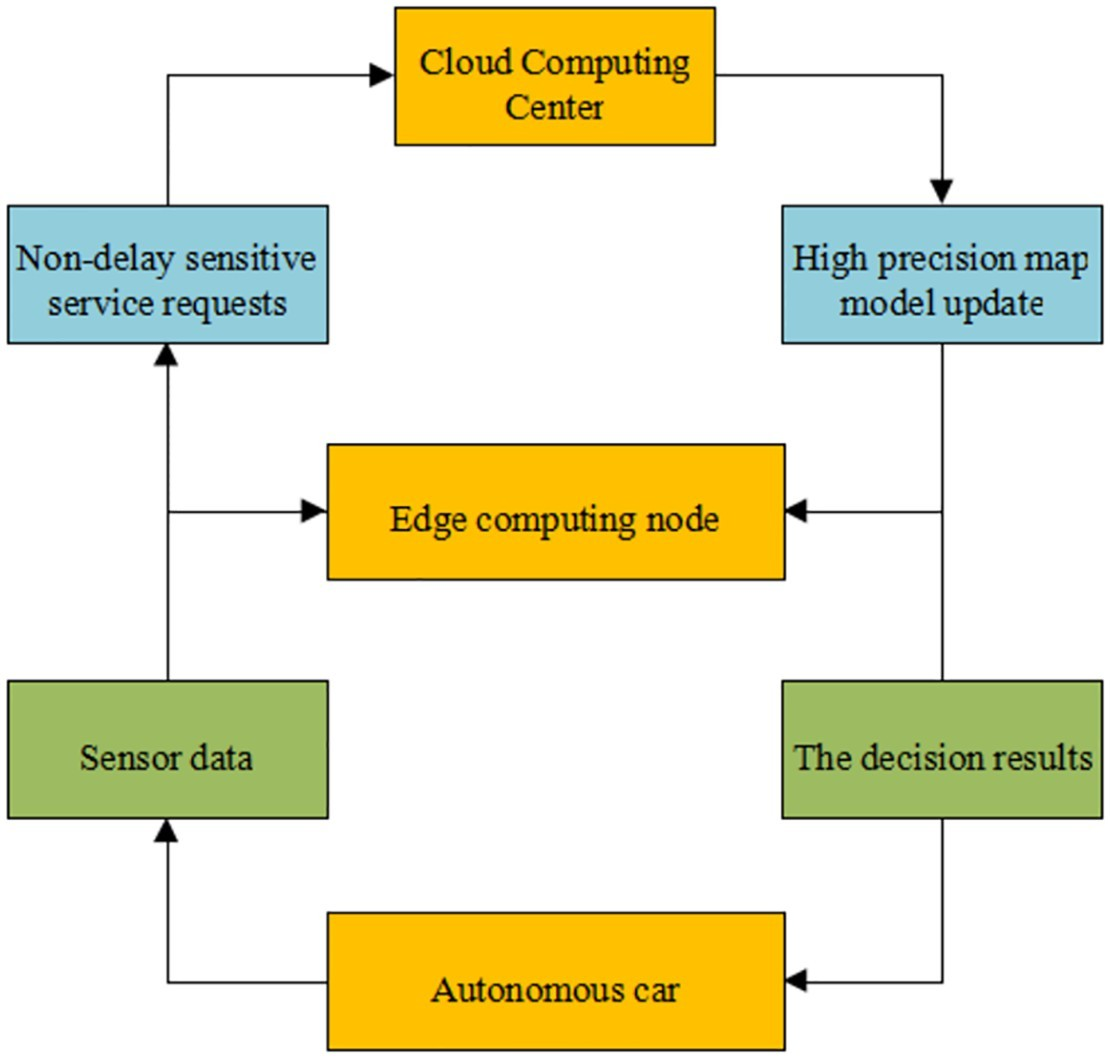
\includegraphics[width=0.72\linewidth]{images/guo2023-edge-av-architecture.jpg}
  \caption[Edge-Computing Architecture for Autonomous Vehicles]{
    Architecture of autonomous vehicles based on edge computing.
    Reproduced from Ming \cite{guo2023}, Fig.~3, under the Creative
    Commons Attribution 4.0 International license (CC BY 4.0).}
  \label{fig:guo-edge-av-architecture}
\end{figure}

\begin{figure}[H]
  \centering
  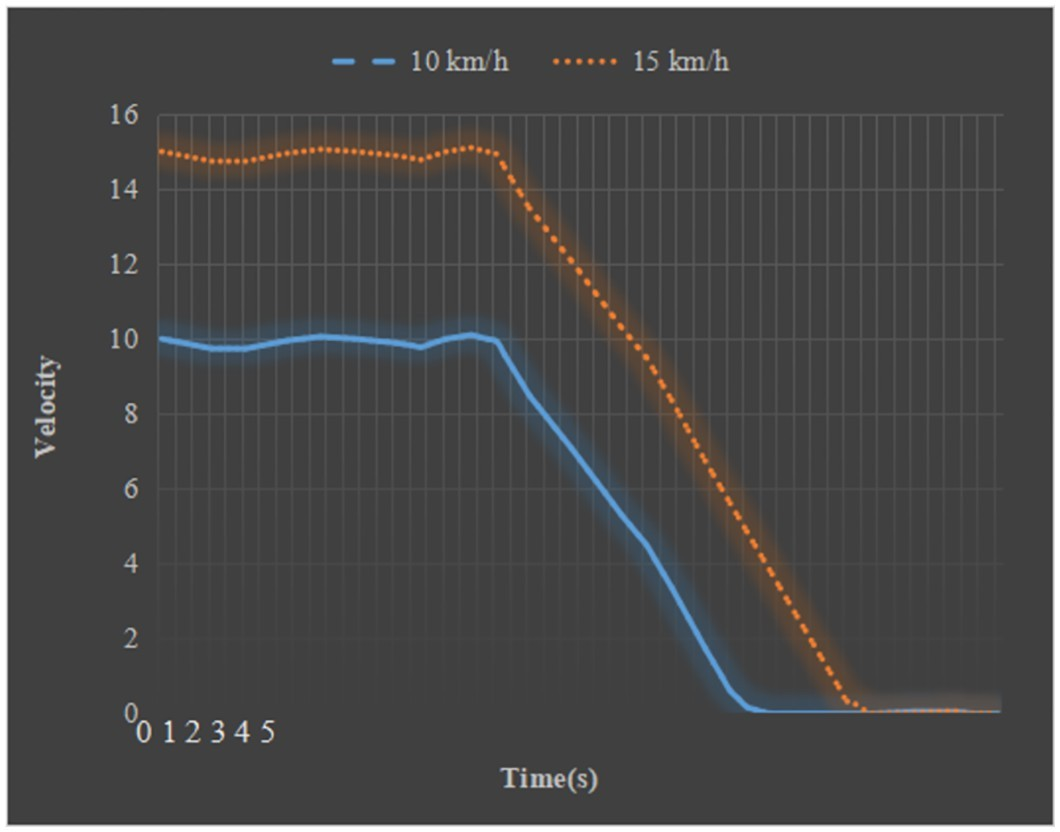
\includegraphics[width=0.78\linewidth]{images/guo2023-emergency-braking-speed.jpg}
  \caption[Emergency-Braking Speed Curves]{
    Emergency-braking speed curves reported by Ming \cite{guo2023},
    Fig.~11. Reproduced under the Creative Commons Attribution 4.0
    International license (CC BY 4.0); these are source-study results,
    not measurements from this project.}
  \label{fig:guo-emergency-braking-speed}
\end{figure}

\chapter{Conclusion and Future Work}

\noindent
Autonomous vehicles were selected because their limited individual sensing
range and occlusions motivate sharing information between connected agents.
The primary technical direction is cooperative perception: onboard
perception provides the local baseline, while selected sensor-derived
features or detection messages may be aligned and fused with V2V or V2I
information. Published studies demonstrate cooperative fusion and
communication-aware feature selection on benchmark datasets, but do not
validate the proposed system over the team's hardware or real vehicle
networks \cite{v2xvit2022,where2comm2022,opv2v2022,cobevt2023}.

Vehicle--edge--cloud collaboration remains relevant as a supporting
architecture. Vehicles perform local perception; roadside edge resources
may relay or process selected cooperative tasks; cloud services handle
longer-term storage, offline training, and model management. The vehicle
must preserve local perception if a peer or edge connection fails or
returns stale information. Communication overhead, latency and freshness,
intermittent links, heterogeneous agents, privacy, and robustness remain
open challenges \cite{v2xsurvey2025,biswas2023}. Federated learning is
retained as a secondary literature direction for future model training,
not part of the primary online prototype \cite{flcav2024}.

The project is now entering Phase 3, Small-Scale Experiments. Initial work
includes CARLA ground-truth camera-label projection in four weather
conditions, three-camera driving-data capture, a 198-frame-per-configuration
detector benchmark, a separate 600-frame demo rerender, and two
steering-model training runs. GPU FP32 detector end-to-end latency was
20.5\,ms mean and 24.2\,ms p95 in its benchmark. The saved steering run did
not outperform an always-straight baseline and achieved 49\% turn-direction
agreement. Next, document the software and hardware configuration, improve
the data and vehicle-only baselines, and continue controlled simulation and
data gathering. Then evaluate cooperative perception and selected edge
offloading, with multi-agent fusion conditional on data, compute, and time.
Measure latency, quality, throughput, communication volume, reliability,
energy where measurable, and resource use under controlled network
conditions. These are preliminary simulator measurements; no real-vehicle
safety or deployment claim is made.

\begin{thebibliography}{99}
  \addcontentsline{toc}{chapter}{References}

  \bibitem{hu2023}
  Fei Hu, Kunal Mehta, Shivakant Mishra, and Mohammad AlMutawa.
  ``Distributed Edge AI Systems.'' In \textit{Proceedings of the IEEE/ACM
  16th International Conference on Utility and Cloud Computing (UCC '23)},
  Taormina, Italy, December 4--7, 2023, pp.\ 1--6.
  \url{https://doi.org/10.1145/3603166.3632546}.

  \bibitem{deng2020}
  Shuiguang Deng, Hailiang Zhao, Weijia Fang, Jianwei Yin, Schahram
  Dustdar, and Albert Y. Zomaya.
  ``Edge Intelligence: The Confluence of Edge Computing and Artificial
  Intelligence.'' \textit{IEEE Internet of Things Journal}, vol.\ 7, no.\ 8,
  pp.\ 7457--7469, August 2020.
  \url{https://doi.org/10.1109/JIOT.2020.2984887}.

  \bibitem{hou2022}
  Xueyu Hou, Yongjie Guan, Tao Han, and Ning Zhang.
  ``DistrEdge: Speeding up Convolutional Neural Network Inference on
  Distributed Edge Devices.'' In \textit{2022 IEEE International Parallel
  and Distributed Processing Symposium (IPDPS)}, Lyon, France, May 30--June 3,
  2022, pp.\ 1097--1107.
  \url{https://doi.org/10.1109/IPDPS53621.2022.00110}.

  \bibitem{mcmahan2017}
  Brendan McMahan, Eider Moore, Daniel Ramage, Seth Hampson, and Blaise
  Aguera y Arcas. ``Communication-Efficient Learning of Deep Networks from
  Decentralized Data.'' In \textit{Proceedings of the 20th International
  Conference on Artificial Intelligence and Statistics}, Proceedings of
  Machine Learning Research, vol.\ 54, pp.\ 1273--1282, 2017.
  \url{https://proceedings.mlr.press/v54/mcmahan17a.html}.

  \bibitem{biswas2023}
  Anushka Biswas and Hwang-Cheng Wang.
  ``Autonomous Vehicles Enabled by the Integration of IoT, Edge Intelligence,
  5G, and Blockchain.'' \textit{Sensors}, vol.\ 23, no.\ 4, article 1963,
  2023. \url{https://doi.org/10.3390/s23041963}.

  \bibitem{flcav2024}
  Vishnu Pandi Chellapandi, Liangqi Yuan, Christopher G. Brinton,
  Stanislaw H. \.{Z}ak, and Ziran Wang.
  ``Federated Learning for Connected and Automated Vehicles: A Survey of
  Existing Approaches and Challenges.'' \textit{IEEE Transactions on
  Intelligent Vehicles}, vol.\ 9, no.\ 1, pp.\ 119--137, 2024.
  \url{https://doi.org/10.1109/TIV.2023.3332675}.

  \bibitem{v2xvit2022}
  Runsheng Xu, Hao Xiang, Zhengzhong Tu, Xin Xia, Ming-Hsuan Yang, and
  Jiaqi Ma. ``V2X-ViT: Vehicle-to-Everything Cooperative Perception with
  Vision Transformer.'' In \textit{Computer Vision -- ECCV 2022},
  Lecture Notes in Computer Science, pp.\ 107--124, 2022.
  \url{https://doi.org/10.1007/978-3-031-19842-7_7}.

  \bibitem{where2comm2022}
  Yue Hu, Shaoheng Fang, Zixing Lei, Yiqi Zhong, and Siheng Chen.
  ``Where2comm: Communication-Efficient Collaborative Perception via
  Spatial Confidence Maps.'' In \textit{Advances in Neural Information
  Processing Systems 35 (NeurIPS 2022)}, pp.\ 4874--4886, 2022.
  \url{https://doi.org/10.52202/068431-0352}.

  \bibitem{opv2v2022}
  Runsheng Xu, Hao Xiang, Xin Xia, Xu Han, Jinlong Li, and Jiaqi Ma.
  ``OPV2V: An Open Benchmark Dataset and Fusion Pipeline for Perception
  with Vehicle-to-Vehicle Communication.'' In \textit{2022 International
  Conference on Robotics and Automation (ICRA)}, pp.\ 2583--2589, 2022.
  \url{https://doi.org/10.1109/ICRA46639.2022.9812038}.

  \bibitem{cobevt2023}
  Runsheng Xu, Zhengzhong Tu, Hao Xiang, Wei Shao, Bolei Zhou, and
  Jiaqi Ma. ``CoBEVT: Cooperative Bird's Eye View Semantic Segmentation
  with Sparse Transformers.'' In \textit{Proceedings of the 6th Conference
  on Robot Learning}, Proceedings of Machine Learning Research, vol.\ 205,
  pp.\ 989--1000, 2023.
  \url{https://proceedings.mlr.press/v205/xu23a.html}.

  \bibitem{v2xsurvey2025}
  Tao Huang, Jianan Liu, Xi Zhou, Dinh C. Nguyen, Mostafa Rahimi Azghadi,
  Yuxuan Xia, Qing-Long Han, and Sumei Sun.
  ``Vehicle-to-Everything Cooperative Perception for Autonomous Driving.''
  \textit{Proceedings of the IEEE}, vol.\ 113, no.\ 5, pp.\ 443--477, 2025.
  \url{https://doi.org/10.1109/JPROC.2025.3600903}.

  \bibitem{coedge2021}
  Liekang Zeng, Xu Chen, Zhi Zhou, Lei Yang, and Junshan Zhang.
  ``CoEdge: Cooperative DNN Inference With Adaptive Workload Partitioning
  Over Heterogeneous Edge Devices.'' \textit{IEEE/ACM Transactions on
  Networking}, vol.\ 29, no.\ 2, pp.\ 595--608, 2021.
  \url{https://doi.org/10.1109/TNET.2020.3042320}.

  \bibitem{guo2023}
  Guo Ming. ``Exploration of the Intelligent Control System of Autonomous
  Vehicles Based on Edge Computing.'' \textit{PLOS ONE}, vol.\ 18, no.\ 2,
  article e0281294, 2023.
  \url{https://doi.org/10.1371/journal.pone.0281294}.
\end{thebibliography}

\end{document}
